% !TEX program = pdflatex
\documentclass[a4paper, 12pt, oneside]{article} %文档设置

% --- 核心宏包加载顺序 ---
\usepackage{enumitem} % 列表宏包,放在 ctex 之前

\usepackage{ctex} % 中文宏包

\usepackage{geometry} % 页面设置
\usepackage{amsmath}  % 数学公式
\usepackage{amssymb}  % 数学符号,如 \mathbb
\usepackage{amsthm}   % !!! 新增:用于支持证明环境 \begin{proof}
	\usepackage{graphicx} % 插图
	\usepackage{multirow} % 表格跨行
	\usepackage{fancyhdr} % 页眉页脚
	\usepackage{titlesec} % 章节标题
	\usepackage{titletoc} % 目录样式
	\usepackage{pdfpages} % 插入PDF
	\usepackage{booktabs} % 美化表格线条
	\usepackage{gbt7714} %参考文献包
	
	% !!! 新增:用于创建算法伪代码框
	\usepackage{algorithm}
	\usepackage{algpseudocode}
	
	% !!! 新增:支持 \captionof
	\usepackage{caption}
	
	% !!! 新增:支持 tikzpicture
	\usepackage{tikz}
	
	\usepackage{hyperref} % 核心:用于创建超链接
	
	% --- 超链接设置 (全部改为黑色) ---
	\hypersetup{
		colorlinks=true,       % 保持链接可点击
		linkcolor=black,        % 内部链接(目录、章节、公式、定理)为蓝色
		citecolor=black,       % 参考文献引用为绿色
		filecolor=black,       % 文件链接为黑色
		urlcolor=black          % 网址链接为青色
	}
	
	\geometry{left = 2.4cm, right = 2.4cm, top = 2.4cm, bottom = 2.4cm} %页面设置
	\linespread{1.5} %行距设置
	
	% --- 章节标题格式设置 (保持不变) ---
	\titleformat*{\section}{\zihao{4} \heiti}
	\titlespacing*{\section}{0pt}{0ex plus 0ex minus 0ex}{0ex plus 0ex}
	\titleformat*{\subsection}{\zihao{-4} \heiti}
	\titlespacing*{\subsection}{0pt}{0ex plus 0ex minus 0ex}{0ex plus 0ex}
	\titleformat*{\subsubsection}{\zihao{-4} \kaishu}
	\titlespacing*{\subsubsection}{0pt}{0ex plus 0ex minus 0ex}{0ex plus 0ex}
	
	% ========== 数学命令 ==========
	\newcommand{\diff}{\mathop{}\!\mathrm{d}}
	\newcommand{\R}{\mathbb{R}}
	\newcommand{\C}{\mathbb{C}}
	\newcommand{\Z}{\mathbb{Z}}
	\newcommand{\N}{\mathbb{N}}
	\DeclareMathOperator{\supp}{supp}
	% 新增:傅里叶和拉普拉斯变换算子
	\newcommand{\F}{\mathcal{F}}
	\newcommand{\Lop}{\mathcal{L}}
	
	% ========== 编号系统 ==========
	\numberwithin{subsection}{section}
	\numberwithin{subsubsection}{subsection}
	\counterwithin{equation}{subsection}
	
	% ========== 定理环境 ==========
	\theoremstyle{plain}
	\newtheorem{theorem}{定理}[section]
	\newtheorem{lemma}[theorem]{引理}
	\newtheorem{proposition}[theorem]{命题}
	\newtheorem{corollary}[theorem]{推论}
	\newtheorem{solution}{解}[subsection]
	
	\theoremstyle{definition}
	\newtheorem{definition}[theorem]{定义}
	\newtheorem{example}{例题}[subsection]
	
	\theoremstyle{remark}
	\newtheorem{remark}[theorem]{注记}
	\newtheorem{verification}{验证}
	
	\begin{document}
		
		% --------------------封面--------------------
		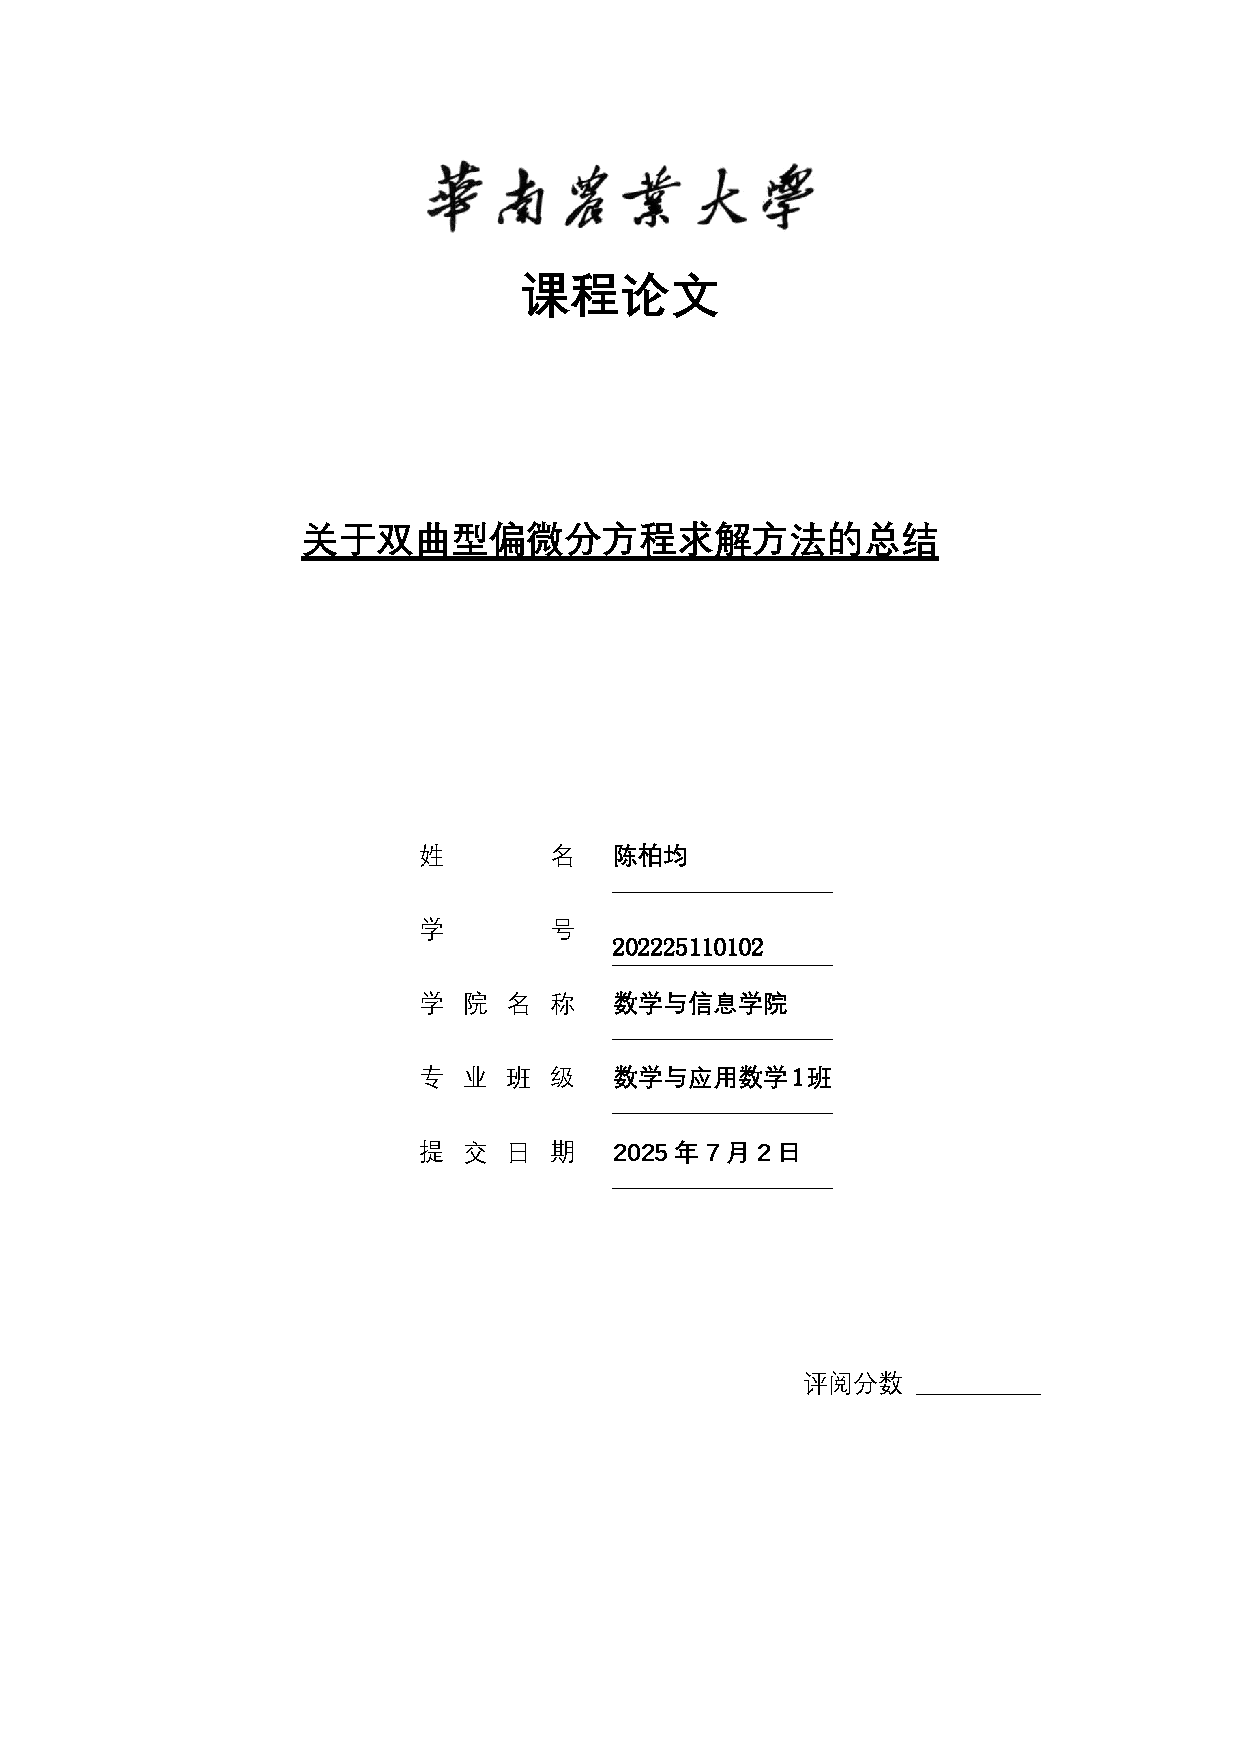
\includepdf[pages=1, pagecommand={\thispagestyle{empty}}]{cover.pdf}
		\clearpage
		
		% --------------------摘要--------------------
		\newpage %分页
		\centerline{\textbf{摘 \quad \quad \quad \quad 要}}
		% --- 修改后的摘要 ---
		本文系统地探讨了二阶线性偏微分方程,特别是双曲型方程的求解策略。首先,文章从特征理论出发,根据判别式 \(\Delta = b^2 - 4ac\) 的符号将二阶线性方程分为双曲型、抛物型和椭圆型,并详细阐述了如何通过特征线进行坐标变换,将双曲型方程化为更易于分析的标准型。
		
		对于线性问题,叠加原理是核心的分解工具。一个复杂的非齐次问题可以被分解为方程非齐次、初始条件非齐次和边界条件非齐次三个(或两个)更简单的子问题。针对这些子问题,本文介绍了两种关键的齐次化技术:第一,对于非齐次边界条件,利用多项式插值的思想构造辅助函数,将其转化为齐次边界条件,但代价是可能引入新的非齐次项和修正初始条件;第二,对于非齐次方程,应用Duhamel原理,将非齐次项的影响转移到初始条件上,从而将问题转化为求解一个参数化的齐次方程族。
		
		在求解核心的齐次方程时,本文根据不同边界条件给出了多种方法。对于无界问题,通过求解传输方程引出求解波动方程的达朗贝尔(d'Alembert)公式。对于有界或半直线上的问题,若满足相容性条件,可通过反射法(奇偶延拓)将问题延拓至全空间,从而继续使用达朗贝尔公式。作为一种更普适的方法,分离变量法被详细介绍,它能系统地处理各种齐次边界条件下的有界问题,通过求解本征值问题将偏微分方程转化为常微分方程组。
		
		
		
		
		% --------------------目录--------------------
		\newpage
		
		\tableofcontents  % 添加目录
		
		
		
		% --------------------正文--------------------
		\newpage
		\songti % 设置正文主要字体为songti
		
		\section{二阶线性偏微分方程按特征分类与标准化}
		\subsection{二阶方程的特征理论}
		考虑两个自变量的二阶拟线性偏微分方程的一般形式:
		\begin{equation}\label{eq:quasi_linear_2nd_order}
			a u_{xx} + b u_{xy} + c u_{yy} = F,
		\end{equation}
		其中系数 \(a, b, c\) 和非齐次项 \(F\) 都是 \(x, y, u, u_x, u_y\) 的已知函数。
		
		假设 \(\Gamma\) 是平面 \(xoy\) 上的一条光滑曲线,我们在这条曲线上给定所谓的 柯西初值条件 ,即函数 \(u\) 及其一阶偏导数的值:
		\begin{equation}\label{eq:cauchy_conditions_general}
			u|_{\Gamma} = \text{已知}, \quad u_x|_{\Gamma} = \text{已知}, \quad u_y|_{\Gamma} = \text{已知}.
		\end{equation}
		这样的定解问题称为 柯西问题 。核心问题是:定解问题 \eqref{eq:quasi_linear_2nd_order} 和 \eqref{eq:cauchy_conditions_general} 的解是否存在且唯一?
		
		为了回答这个问题,我们退一步思考:能否根据给定的方程和初值条件,唯一地确定解的所有二阶偏导数 \(u_{xx}, u_{xy}, u_{yy}\) 在曲线 \(\Gamma\) 上的值?如果连二阶导数都无法确定,解的存在唯一性就无从谈起。
		
		设曲线 \(\Gamma\) 的参数方程为 \(x = \varphi(s), y = \psi(s)\)。那么,柯西条件 \eqref{eq:cauchy_conditions_general} 可以更具体地写为:
		\begin{equation}\label{eq:cauchy_conditions_parametric}
			\begin{cases}
				u|_{\Gamma} = u(\varphi(s), \psi(s)) = u^0(s), \\
				u_x|_{\Gamma} = u_x(\varphi(s), \psi(s)) = p^0(s), \\
				u_y|_{\Gamma} = u_y(\varphi(s), \psi(s)) = q^0(s),
			\end{cases}
		\end{equation}
		其中 \(u^0(s), p^0(s), q^0(s)\) 是已知的函数。
		
		首先,这三个给定的函数并非完全独立。对 \eqref{eq:cauchy_conditions_parametric} 中第一个式子沿曲线 \(\Gamma\) 对参数 \(s\) 求导,根据链式法则有:
		\[
		\frac{\diff u^0(s)}{\diff s} = \frac{\partial u}{\partial x} \frac{\diff x}{\diff s} + \frac{\partial u}{\partial y} \frac{\diff y}{\diff s} = u_x \varphi'(s) + u_y \psi'(s).
		\]
		将 \(u_x\) 和 \(u_y\) 在 \(\Gamma\) 上的值代入,我们得到如下的相容性条件 :
		\begin{equation}
			(u^0(s))' = p^0(s)\varphi'(s) + q^0(s)\psi'(s).
		\end{equation}
		这表明初始数据必须满足此条件。
		
		接下来,为了求出二阶导数,我们自然地想到对 \eqref{eq:cauchy_conditions_parametric} 中的后两个式子也沿 \(\Gamma\) 对 \(s\) 求导:
		\begin{align}
			(p^0(s))' = \frac{\diff u_x}{\diff s} &= u_{xx}\varphi'(s) + u_{xy}\psi'(s), \label{eq:deriv_eq1} \\
			(q^0(s))' = \frac{\diff u_y}{\diff s} &= u_{yx}\varphi'(s) + u_{yy}\psi'(s). \label{eq:deriv_eq2}
		\end{align}
		假设解 \(u\) 是二次连续可微的,即 \(u_{xy} = u_{yx}\)。现在,我们将方程 \eqref{eq:quasi_linear_2nd_order} 本身(在曲线 \(\Gamma\) 上成立)与上面两个求导得到的式子 \eqref{eq:deriv_eq1}、\eqref{eq:deriv_eq2} 联立,得到一个关于三个未知量 \(u_{xx}, u_{xy}, u_{yy}\) 的线性方程组:
		\begin{equation}
			\begin{cases}
				a u_{xx} + b u_{xy} + c u_{yy} = F, \\
				\varphi'(s) u_{xx} + \psi'(s) u_{xy} = (p^0(s))', \\
				\varphi'(s) u_{xy} + \psi'(s) u_{yy} = (q^0(s))'.
			\end{cases}
		\end{equation}
		这个线性系统的系数行列式 \(D\) 为:
		\begin{equation}
			D = 
			\begin{vmatrix}
				a & b & c \\
				\varphi' & \psi' & 0 \\
				0 & \varphi' & \psi'
			\end{vmatrix}
			= a(\psi')^2 - b\varphi'\psi' + c(\varphi')^2.
		\end{equation}
		
		\begin{definition}[特征曲线]
			\begin{enumerate}[label=(\roman*)]
				\item 如果行列式 \(D \neq 0\),则线性方程组有唯一解。这意味着我们可以在曲线 \(\Gamma\) 上唯一地确定所有二阶偏导数的值。这样的曲线 \(\Gamma\) 称为方程 \eqref{eq:quasi_linear_2nd_order} 的非特征曲线。
				\item 如果行列式 \(D = 0\),则线性方程组的解不是唯一的(可能有无穷多解或无解,取决于右侧的常数项)。这意味着我们无法在 \(\Gamma\) 上唯一确定二阶导数。这样的曲线 \(\Gamma\) 称为方程 \eqref{eq:quasi_linear_2nd_order} 的特征曲线 。
			\end{enumerate}
		\end{definition}
		
		特征曲线满足的方程 \(D=0\) 称为特征方程 :
		\begin{equation}\label{eq:characteristic_eq_parametric}
			a(\psi'(s))^2 - b\varphi'(s)\psi'(s) + c(\varphi'(s))^2 = 0.
		\end{equation}
		注意到 \(\varphi'(s) = \frac{\diff x}{\diff s}\) 且 \(\psi'(s) = \frac{\diff y}{\diff s}\)。用 \((\diff s)^2\) 除以上式,并考虑到在特征曲线上 \(\frac{\diff y}{\diff x} = \frac{\psi'(s)}{\varphi'(s)}\),我们得到特征方程的微分形式:
		\begin{equation}\label{eq:characteristic_ode}
			a \left(\frac{\diff y}{\diff x}\right)^2 - b \frac{\diff y}{\diff x} + c = 0.
		\end{equation}
		这是一个关于 \(\frac{\diff y}{\diff x}\) 的二次方程,解出它就得到了特征曲线的斜率。
		
		
		\subsection{方程的分类与标准型}
		二阶线性方程的分类是基于特征方程的性质,这在可逆的自变量变换下是不变的。我们主要根据判别式 \(\Delta = b^2 - 4ac\) 的符号来分类。
		\begin{definition}[方程的分类]
			对于方程 \eqref{eq:quasi_linear_2nd_order}(这里我们考虑系数 \(a,b,c\) 仅依赖于 \(x,y\) 的线性情况),在某一点 \((x,y)\) 定义其判别式为 \(\Delta = b^2 - 4ac\)。
			\begin{itemize}
				\item 若 \(\Delta(x,y) > 0\),称方程在该点是双曲型 。
				\item 若 \(\Delta(x,y) = 0\),称方程在该点是抛物型 。
				\item 若 \(\Delta(x,y) < 0\),称方程在该点是椭圆型。
			\end{itemize}
		\end{definition}
		通过选择恰当的自变量变换,可以将方程化为最简形式,即标准型。这个变换的关键是利用特征曲线作为新的坐标线。
		
		\subsubsection{双曲型方程 (\texorpdfstring{$\Delta > 0$}{Delta > 0})}
		当 \(\Delta > 0\) 时,特征方程 \eqref{eq:characteristic_ode} 有两个不同的实数解,对应两族实特征曲线。
		\[
		\frac{\diff y}{\diff x} = \frac{b + \sqrt{b^2-4ac}}{2a} \quad \text{和} \quad \frac{\diff y}{\diff x} = \frac{b - \sqrt{b^2-4ac}}{2a}.
		\]
		积分这两组常微分方程,得到两族特征曲线 \(\varphi(x,y) = c_1\) 和 \(\psi(x,y) = c_2\)。
		我们选取新的坐标变换:
		\[
		\xi = \varphi(x,y), \quad \eta = \psi(x,y).
		\]
		在此变换下,可以证明新坐标系下的系数 \(A=0\) 且 \(C=0\),而 \(B \neq 0\)。原方程化为:
		\begin{equation}\label{eq:hyperbolic_canonical_1}
			u_{\xi\eta} + (\text{低阶项}) = 0.
		\end{equation}
		这称为双曲型方程的第一标准型。如果再做一个线性变换 \(\tilde{x} = \xi+\eta, \tilde{y}=\xi-\eta\),则可以消去混合偏导项,得到:
		\begin{equation}\label{eq:hyperbolic_canonical_2}
			u_{\tilde{x}\tilde{x}} - u_{\tilde{y}\tilde{y}} + (\text{低阶项}) = 0.
		\end{equation}
		这称为双曲型方程的第二标准型,典型的例子就是波动方程。
		
		\begin{proof}[第一标准型变换验证]
			我们来验证,当选取特征曲线 \(\varphi(x,y)=c_1\) 和 \(\psi(x,y)=c_2\) 作为新坐标 \(\xi=\varphi(x,y)\) 和 \(\eta=\psi(x,y)\) 时,新方程的系数 \(A\) 和 \(C\) 确实为零。
			
			在新坐标系下,二阶偏导项的系数为:
			\begin{align*}
				A &= a\varphi_x^2 + b\varphi_x\varphi_y + c\varphi_y^2 \\
				B &= a\varphi_x\psi_x + \frac{b}{2}(\varphi_x\psi_y + \varphi_y\psi_x) + c\varphi_y\psi_y \\
				C &= a\psi_x^2 + b\psi_x\psi_y + c\psi_y^2
			\end{align*}
			
			由于 \(\varphi(x,y)=c_1\) 是一条特征曲线,它的梯度向量 \((\varphi_x, \varphi_y)\) 与曲线的切线方向 \((\diff x, \diff y)\) 正交,即 \(\varphi_x \diff x + \varphi_y \diff y = 0\),所以 \(\frac{\diff y}{\diff x} = -\frac{\varphi_x}{\varphi_y}\)。
			
			将此代入特征方程 \eqref{eq:characteristic_ode}:
			\[
			a \left(-\frac{\varphi_x}{\varphi_y}\right)^2 - b \left(-\frac{\varphi_x}{\varphi_y}\right) + c = 0
			\]
			两边同乘以 \(\varphi_y^2\)(假设 \(\varphi_y \neq 0\)),得到:
			\[
			a\varphi_x^2 + b\varphi_x\varphi_y + c\varphi_y^2 = 0.
			\]
			这正是新系数 \(A\) 的表达式。因此,\(A=0\)。
			
			同理,由于 \(\psi(x,y)=c_2\) 也是一条特征曲线,可证 \(C=0\)。
			
			对于系数 \(B\),由于 \(\varphi\) 和 \(\psi\) 来自两个不同的特征根,它们是线性无关的,可以证明 \(B \neq 0\)。因此,方程成功化为只含混合偏导数 \(u_{\xi\eta}\) 的第一标准型。
		\end{proof}
		
		\begin{proof}[第二标准型变换验证]
			我们从双曲型方程的第一标准型出发:
			\[
			u_{\xi\eta} + D_0 u_\xi + E_0 u_\eta + G_0 u = F_0.
			\]
			引入新的线性变换:
			\[
			\tilde{x} = \xi + \eta, \quad \tilde{y} = \xi - \eta.
			\]
			反过来,我们有 \(\xi = \frac{1}{2}(\tilde{x}+\tilde{y})\) 和 \(\eta = \frac{1}{2}(\tilde{x}-\tilde{y})\)。
			
			我们的目标是计算 \(u_{\xi\eta}\) 如何用新坐标 \((\tilde{x}, \tilde{y})\) 的偏导数来表示。首先,使用链式法则计算一阶导数:
			\begin{align*}
				u_\xi &= \frac{\partial u}{\partial \xi} = \frac{\partial u}{\partial \tilde{x}}\frac{\partial \tilde{x}}{\partial \xi} + \frac{\partial u}{\partial \tilde{y}}\frac{\partial \tilde{y}}{\partial \xi} = u_{\tilde{x}} \cdot 1 + u_{\tilde{y}} \cdot 1 = u_{\tilde{x}} + u_{\tilde{y}}, \\
				u_\eta &= \frac{\partial u}{\partial \eta} = \frac{\partial u}{\partial \tilde{x}}\frac{\partial \tilde{x}}{\partial \eta} + \frac{\partial u}{\partial \tilde{y}}\frac{\partial \tilde{y}}{\partial \eta} = u_{\tilde{x}} \cdot 1 + u_{\tilde{y}} \cdot (-1) = u_{\tilde{x}} - u_{\tilde{y}}.
			\end{align*}
			
			接下来,计算混合偏导数 \(u_{\xi\eta}\)。我们将算子 \(\frac{\partial}{\partial \eta}\) 作用于 \(u_\xi\):
			\begin{align*}
				u_{\xi\eta} = \frac{\partial}{\partial \eta}(u_\xi) &= \frac{\partial}{\partial \eta}(u_{\tilde{x}} + u_{\tilde{y}}) \\
				&= \frac{\partial (u_{\tilde{x}})}{\partial \eta} + \frac{\partial (u_{\tilde{y}})}{\partial \eta}.
			\end{align*}
			再次应用链式法则:
			\begin{align*}
				\frac{\partial (u_{\tilde{x}})}{\partial \eta} &= \frac{\partial (u_{\tilde{x}})}{\partial \tilde{x}}\frac{\partial \tilde{x}}{\partial \eta} + \frac{\partial (u_{\tilde{x}})}{\partial \tilde{y}}\frac{\partial \tilde{y}}{\partial \eta} = u_{\tilde{x}\tilde{x}} \cdot 1 + u_{\tilde{x}\tilde{y}} \cdot (-1) = u_{\tilde{x}\tilde{x}} - u_{\tilde{x}\tilde{y}}, \\
				\frac{\partial (u_{\tilde{y}})}{\partial \eta} &= \frac{\partial (u_{\tilde{y}})}{\partial \tilde{x}}\frac{\partial \tilde{x}}{\partial \eta} + \frac{\partial (u_{\tilde{y}})}{\partial \tilde{y}}\frac{\partial \tilde{y}}{\partial \eta} = u_{\tilde{y}\tilde{x}} \cdot 1 + u_{\tilde{y}\tilde{y}} \cdot (-1) = u_{\tilde{y}\tilde{x}} - u_{\tilde{y}\tilde{y}}.
			\end{align*}
			将这两部分加起来,并利用 \(u_{\tilde{x}\tilde{y}} = u_{\tilde{y}\tilde{x}}\),我们得到:
			\[
			u_{\xi\eta} = (u_{\tilde{x}\tilde{x}} - u_{\tilde{x}\tilde{y}}) + (u_{\tilde{y}\tilde{x}} - u_{\tilde{y}\tilde{y}}) = u_{\tilde{x}\tilde{x}} - u_{\tilde{y}\tilde{y}}.
			\]
			
			现在,将 \(u_{\xi\eta}\), \(u_\xi\), 和 \(u_\eta\) 的新表达式代回第一标准型方程:
			\[
			(u_{\tilde{x}\tilde{x}} - u_{\tilde{y}\tilde{y}}) + D_0(u_{\tilde{x}} + u_{\tilde{y}}) + E_0(u_{\tilde{x}} - u_{\tilde{y}}) + G_0 u = F_0.
			\]
			整理后得到:
			\[
			u_{\tilde{x}\tilde{x}} - u_{\tilde{y}\tilde{y}} + (D_0+E_0)u_{\tilde{x}} + (D_0-E_0)u_{\tilde{y}} + G_0 u = F_0.
			\]
			这是一个只包含 \(u_{\tilde{x}\tilde{x}}\) 和 \(u_{\tilde{y}\tilde{y}}\) 作为二阶项的形式,即双曲型方程的第二标准型。
		\end{proof}
		\begin{remark}
			化为第二标准型就是我们的波动方程,由达朗贝尔公式可知,双曲线方程可以写成第二标准型后两条特征线变量的组合,而且特征线变量不会杂糅到一起。
			\[
			u(\xi, \eta) = F(\xi) + G(\eta)
			\]
		\end{remark}
		
		
		\begin{example}
			判断下列方程的类型,并化成标准型:
			\[ 3u_{xx} + 2u_{xy} - u_{yy} + u_x + u_y = 0. \]
		\end{example}
		\begin{solution}
			步骤1. 判断类型
			
			系数 $A=3, B=2, C=-1$。判别式 $\Delta = B^2 - 4AC = 2^2 - 4(3)(-1) = 4+12=16>0$。方程为双曲型。
			
			步骤2. 求解特征方程
			
			特征方程为 $A(\frac{dy}{dx})^2 - B\frac{dy}{dx} + C = 0 \implies 3(\frac{dy}{dx})^2 - 2\frac{dy}{dx} - 1 = 0$。
			分解得 $(3\frac{dy}{dx}+1)(\frac{dy}{dx}-1)=0$。
			特征方向为 $\lambda_1 = 1$ 和 $\lambda_2 = -1/3$。
			对应的特征线方程为 $y-x=C_1$ 和 $y+\frac{1}{3}x=C_2$ (或 $3y+x=C_2$)。
			
			步骤3. 进行坐标变换
			
			取新坐标 $\xi = y-x, \eta=3y+x$。计算偏导数:
			\begin{align*}
				u_x &= u_\xi \xi_x + u_\eta \eta_x = -u_\xi + u_\eta \\
				u_y &= u_\xi \xi_y + u_\eta \eta_y = u_\xi + 3u_\eta \\
				u_{xx} &= \frac{\partial}{\partial x}(-u_\xi + u_\eta) = -(-u_{\xi\xi} + u_{\xi\eta}) + (-u_{\eta\xi} + u_{\eta\eta}) = u_{\xi\xi} - 2u_{\xi\eta} + u_{\eta\eta} \\
				u_{xy} &= \frac{\partial}{\partial y}(-u_\xi + u_\eta) = -(u_{\xi\xi} + 3u_{\xi\eta}) + (u_{\eta\xi} + 3u_{\eta\eta}) = -u_{\xi\xi} - 2u_{\xi\eta} + 3u_{\eta\eta} \\
				u_{yy} &= \frac{\partial}{\partial y}(u_\xi + 3u_\eta) = (u_{\xi\xi} + 3u_{\xi\eta}) + 3(u_{\eta\xi} + 3u_{\eta\eta}) = u_{\xi\xi} + 6u_{\xi\eta} + 9u_{\eta\eta}
			\end{align*}
			
			步骤4. 代入原方程化简
			
			二阶项: $3u_{xx} + 2u_{xy} - u_{yy} = 3(u_{\xi\xi} - 2u_{\xi\eta} + u_{\eta\eta}) + 2(-u_{\xi\xi} - 2u_{\xi\eta} + 3u_{\eta\eta}) - (u_{\xi\xi} + 6u_{\xi\eta} + 9u_{\eta\eta}) = (3-2-1)u_{\xi\xi} + (-6-4-6)u_{\xi\eta} + (3+6-9)u_{\eta\eta} = -16u_{\xi\eta}$。
			
			一阶项: $u_x + u_y = (-u_\xi + u_\eta) + (u_\xi + 3u_\eta) = 4u_\eta$。
			
			合并得到 $-16u_{\xi\eta} + 4u_\eta = 0$。两边同除以 $-4$,得到标准型:
			\[ 4u_{\xi\eta} - u_\eta = 0 \]
		\end{solution}
		
		
		
		\section{按边界条件分类偏微分方程}
		一般的偏微分方程是由空间变量$x \in \R$和时间变量$t \geq 0$构成的问题,有三个条件:方程,初始条件($t=0$),边界条件($x=0, \quad l=0$).
		
		根据空间变量$x$的范围,即边界条件可以分类成三类问题,再根据每类问题的边界条件是原函数还是一阶导函数可分类子问题7个。
		
		下面用波动方程举例,方程原则上可以算任意方程。
		\subsection{有界}
		有界指的是空间变量$x \in [0,l]$和时间变量$t \geq 0$.
		
		$x=0,\quad l=0$都有函数,可能都是原函数(第一类边界,也叫Dirichlet边界条件);可能都是一阶导函数(第二类边界);可能一个是原函数,另一个是一阶偏导函数(混合边界,有两个)。
		\subsubsection{第一类边界}
		$x=0,\quad l=0$都是原函数。
		\begin{equation}\label{eq:wave_bounded_dirichlet}
			\begin{cases}
				u_{tt} - a^2 u_{xx} = f(x, t), & 0 < x < l, \ t > 0, \\
				u(x, 0) = \varphi(x), \ u_t(x, 0) = \psi(x), & 0 \leq x \leq l, \\
				u(0, t) = \mu_1(t), \ u(l, t) = \mu_2(t), & t \geq 0.
			\end{cases}
		\end{equation}
		\subsubsection{第二类边界}
		$x=0,\quad l=0$都是一阶偏导函数。
		\begin{equation}\label{eq:wave_bounded_neumann}
			\begin{cases}
				u_{tt} - a^2 u_{xx} = f(x, t), & 0 < x < l, \ t > 0, \\
				u(x, 0) = \varphi(x), \ u_t(x, 0) = \psi(x), & 0 \leq x \leq l, \\
				u_x(0, t) = \mu_1(t), \ u_x(l, t) = \mu_2(t), & t \geq 0.
			\end{cases}
		\end{equation}
		
		
		\subsubsection{两种混合}
		第一种:$x=0$处是原函数,$ l=0$是一阶偏导函数。
		\begin{equation}\label{eq:wave_bounded_mixed1}
			\begin{cases}
				u_{tt} - a^2 u_{xx} = f(x, t), & 0 < x < l, \ t > 0, \\
				u(x, 0) = \varphi(x), \ u_t(x, 0) = \psi(x), & 0 \leq x \leq l, \\
				u(0, t) = \mu_1(t), \ u_x(l, t) = \mu_2(t), & t \geq 0.
			\end{cases}
		\end{equation}
		
		第二种:$x=0$处是一阶偏导函数,$ l=0$是原函数。
		\begin{equation}\label{eq:wave_bounded_mixed2}
			\begin{cases}
				u_{tt} - a^2 u_{xx} = f(x, t), & 0 < x < l, \ t > 0, \\
				u(x, 0) = \varphi(x), \ u_t(x, 0) = \psi(x), & 0 \leq x \leq l, \\
				u_x(0, t) = \mu_1(t), \ u(l, t) = \mu_2(t), & t \geq 0.
			\end{cases}
		\end{equation}
		
		
		
		\subsection{半直线}
		半直线指空间变量$x \geq 0$,时间变量$t \geq 0$
		
		故边界条件只有$x=0$一个,再根据第一边界,第二边界就可以分成两类。
		\subsubsection{第一边界}
		\begin{equation}\label{eq:wave_half_dirichlet}
			\begin{cases}
				u_{tt} - a^2 u_{xx} = f(x, t), & x > 0, \ t > 0, \\
				u(x, 0) = \varphi(x), \ u_t(x, 0) = \psi(x), & x > 0, \\
				u(0, t) = \mu_1(t), & t \geq 0.
			\end{cases}
		\end{equation}
		
		\subsubsection{第二边界}
		\begin{equation}\label{eq:wave_half_neumann}
			\begin{cases}
				u_{tt} - a^2 u_{xx} = f(x, t), &  x > 0, \ t > 0, \\
				u(x, 0) = \varphi(x), \ u_t(x, 0) = \psi(x), & x > 0, \\
				u_x(0, t) = \mu_1(t), & t \geq 0.
			\end{cases}
		\end{equation}
		
		\subsection{无界}
		
		\begin{equation}\label{eq:wave_unbounded}
			\begin{cases}
				u_{tt} - a^2 u_{xx} = f(x, t), &  x \in (-\infty , +\infty), \ t > 0, \\
				u(x, 0) = \varphi(x), \ u_t(x, 0) = \psi(x), & x \in (-\infty , +\infty) \\
			\end{cases}
		\end{equation}
		
		

		\section{叠加原理}
		叠加原理是一种思想,和分离变量法一样。对于三个非齐次条件都是线性的,就可以分解成三个方程的叠加。下面举第一边界条件的有界波动方程做例子.
		
		对于问题\eqref{eq:wave_bounded_dirichlet},我们可以使用叠加原理将其分解为3个子问题.
		\subsection{方程非齐次}
		\begin{equation}\label{eq:subproblem1}
			\begin{cases}
				u_{tt} - a^2 u_{xx} = f(x, t), & 0 < x < l, \ t > 0, \\
				u(x, 0) = 0, \ u_t(x, 0) = 0, & 0 \leq x \leq l, \\
				u(0, t) = 0, \ u(l, t) = 0, & t \geq 0.
			\end{cases}
		\end{equation}
		\begin{remark}
			对于方程\eqref{eq:subproblem1}我们用Duhamamel原理,将方程齐次化,方程的函数转移到初始条件最高偏导函数上,与7个边界条件没有关系,化成方程\eqref{eq:subproblem2}.
		\end{remark}
		
		\subsection{初始条件非齐次}
		\begin{equation}\label{eq:subproblem2}
			\begin{cases}
				u_{tt} - a^2 u_{xx} = 0, & 0 < x < l, \ t > 0, \\
				u(x, 0) = \varphi(x), \ u_t(x, 0) = \psi(x), & 0 \leq x \leq l, \\
				u(0, t) = 0, \ u(l, t) = 0, & t \geq 0.
			\end{cases}
		\end{equation}
		\begin{remark}
			这个也是最基础的方程,方程\eqref{eq:subproblem1}和\eqref{eq:subproblem3}都可以齐次化成这样的方程,故这个方程是我们最终要解决的方程。
		\end{remark}
		
		
		\subsection{边界条件非齐次}
		\begin{equation}\label{eq:subproblem3}
			\begin{cases}
				u_{tt} - a^2 u_{xx} = 0, & 0 < x < l, \ t > 0, \\
				u(x, 0) = 0, \ u_t(x, 0) = 0, & 0 \leq x \leq l, \\
				u(0, t) = \mu_1(t), \ u(l, t) = \mu_2(t), & t \geq 0.
			\end{cases}
		\end{equation}	
		
		通过数值分析中的线性插值可以把任何边界条件其次化,转化成下面的方程:
		\begin{equation}\label{eq:subproblem3_homogenized}
			\begin{cases}
				v_{tt} - a^2 v_{xx} = f_1(x, t), & 0 < x < l, \ t > 0, \\
				v|_{t=0} = \varphi_1(x), \quad v_t|_{t=0} = \psi_1(x), & 0 \leq x \leq l, \\
				v|_{x=0} = 0, \quad v|_{x=l} = 0, & t \geq 0.
			\end{cases}
		\end{equation}
		
		
		\begin{remark}
			对于问题\eqref{eq:subproblem3_homogenized},我们可以使用叠加原理将其分解为两个子问题,又回到上面的两个方程\eqref{eq:subproblem1}和\eqref{eq:subproblem2}
		\end{remark}
		
		
		
		
		\newpage
		
		\section{边界条件齐次化}
		本质上就是数值分析上的插值。知道两个端点的信息或者一个点的信息,用函数拟合插值。我这里不需要拟合,原则上可以选取任意满足边界条件的函数,为了方便后面的方程计算,我们一般选取牛顿插值法,即多项式插值。	
		
		因为我们只有两个条件,但是如果是多次,比如四次的多项式有4个未知数,而这些未知数我们可以随便取,故我们一般为简化后面的计算,让待定的最高的系数为0(原则上我们取多少次多项式都可以,但是为了后面的计算我们肯定是想让次数最低)
		
		第一边界条件两个都是原函数,明显用一次,两个参数就可以被确定;第二边界条件两个都是导函数,明显用二次多项式,求导后为一次,两个参数可根据导函数确定;故混合边界条件一定不会超过二次。所以我们干脆混合边界条件直接全部取二次就好了,到时候让最高次待定系数为0就好(如果你看了后面,其实都是一次,我这里只是为了思路通畅)
		\subsection{第一边界条件齐次化}
		要想利用Duhamamel原理,我们首先将第一边界条件齐次化,即要找到一个恰当的变换将第一边界值变为零。
		对于第一类边界条件的有界波动方程\eqref{eq:wave_bounded_dirichlet}:
		
		由边界条件
		\begin{equation}
			u(0,t) = \mu_1(t), \quad u(l,t) = \mu_2(t), \quad t \geq 0.
		\end{equation}
		
		设$U(x, t)=ax+b$
		\[
		\begin{cases}
			u(0, t) = \mu_1(t) = U(0, t) = b, \\
			u(l, t) = \mu_2(t) = U(l, t) = al + \mu_1(t),
		\end{cases}
		\]
		\[
		\begin{cases}
			a = \frac{1}{l}(\mu_2(t) - \mu_1(t)), \\
			b = \mu_1(t).
		\end{cases}
		\]
		对方程 \eqref{eq:wave_bounded_dirichlet}构造关于变量 \(x\) 的线性辅助函数(直线方程):
		\begin{equation}
			U(x, t) = \mu_1(t) + \frac{x}{l}(\mu_2(t) - \mu_1(t)),
		\end{equation}
		
		作变换:
		\begin{equation}
			v(x, t) = u(x, t) - U(x, t),
		\end{equation}
		
		代入方程\eqref{eq:wave_bounded_dirichlet},
		得到方程\eqref{eq:homogenized_A}:
		\begin{equation}\label{eq:homogenized_A}
			\begin{cases}
				v_{tt} - a^2 v_{xx} = f_1(x, t), & 0 < x < l, \ t > 0, \\
				v(x, 0) = \varphi_1(x), \quad v_t(x, 0) = \psi_1(x), & 0 \leq x \leq l, \\
				v(0, t) = 0, \quad v(l, t) = 0. &
			\end{cases}
		\end{equation}
		其中:
		\begin{equation}
			\begin{cases}
				f_1(x, t) = f(x, t) - \mu_1''(t) - \frac{x}{l}(\mu_2''(t) - \mu_1''(t)), \\
				\varphi_1(x) = \varphi(x) - \mu_1(0) - \frac{x}{l}(\mu_2(0) - \mu_1(0)), \\
				\psi_1(x) = \psi(x) - \mu_1'(0) - \frac{x}{l}(\mu_2'(0) - \mu_1'(0)).
			\end{cases}
		\end{equation}
		
		这样我们就完成了第一边界条件的齐次化。
		
		\subsection{第二边界条件齐次化}
		为利用Duhamel原理,需将非齐次Neumann边界条件齐次化,即构造变换使边界导数归零。
		
		
		以下我们仅考虑如下第二边界条件的有界波动方程\eqref{eq:wave_bounded_neumann}:
		
		设$U(x, t)=ax^2+bx+c$
		\[
		\begin{cases}
			u_x(0, t) = \mu_1(t) = U_x(0, t) = b, \\
			u_x(l, t) = \mu_2(t) = U_x(l, t) = 2al + b,
		\end{cases}
		\]
		\[
		\begin{cases}
			a = \frac{1}{2l}(\mu_2(t) - \mu_1(t)) \\
			b = \mu_1(t) \\
			c = 0 
		\end{cases}
		\]
		
		构造辅助函数:
		\begin{equation}
			U(x, t) = x\mu_1(t) + \frac{x^2}{2l}\big( \mu_2(t) - \mu_1(t) \big),
		\end{equation}
		
		作变换:
		\begin{equation}
			v(x, t) = u(x, t) - U(x, t),
		\end{equation}
		
		代入原方程\eqref{eq:wave_bounded_neumann},
		得到方程\eqref{eq:homogenized_B}:
		\begin{equation}\label{eq:homogenized_B}
			\begin{cases}
				v_{tt} - a^2 v_{xx} = f_2(x, t), & 0 < x < l, \ t > 0, \\
				v(x, 0) = \varphi_2(x), \quad v_t(x, 0) = \psi_2(x), & 0 \leq x \leq l, \\
				v_x(0, t) = 0, \quad v_x(l, t) = 0. &
			\end{cases}
		\end{equation}
		
		其中:
		\begin{equation}
			\begin{cases}
				f_2(x, t) = f(x, t)-x\mu_1''(t) - \frac{x^2}{2l}\big( \mu_2''(t) - \mu_1''(t) \big) + \frac{a^2}{l}\big( \mu_2(t) - \mu_1(t) \big), \\
				\varphi_2(x) = \varphi(x) - x\mu_1(0) - \frac{x^2}{2l}\big( \mu_2(0) - \mu_1(0) \big), \\
				\psi_2(x) = \psi(x) - x\mu_1'(0) - \frac{x^2}{2l}\big( \mu_2'(0) - \mu_1'(0) \big), 
			\end{cases}
		\end{equation}
		
		
		
		\subsection{第一混合边界条件齐次化}
		本质上就是数值分析上的插值,原理同上。
		对于问题\eqref{eq:wave_bounded_mixed1}
		
		由边界条件
		\begin{equation}
			u(0,t) = \mu_1(t), \quad u_x(l,t) = \mu_2(t), \quad t \geq 0.
		\end{equation}
		
		设$u(x, t)=U(x, t)=ax^2+bx+c$
		\[
		\begin{cases}
			u(0, t) = \mu_1(t) = U(0, t) = c, \\
			u_x(l, t) = \mu_2(t) = U_x(l, t) = 2al + b,
		\end{cases}
		\]
		\[
		\begin{cases}
			a = 0 (\text{令最高次待定系数为0})\\
			b =\mu_2(t) \\
			c = \mu_1(t)
		\end{cases}
		\]
		
		对方程 \eqref{eq:wave_bounded_mixed1}构造关于变量 \(x\) 的线性辅助函数(直线方程):
		\begin{equation}
			U(x, t) =  \mu_2(t) x+\mu_1(t) ,
		\end{equation}
		
		作变换:
		\begin{equation}
			v(x, t) = u(x, t) - U(x, t),
		\end{equation}
		
		代入方程\eqref{eq:wave_bounded_mixed1},
		得到方程\eqref{eq:homogenized_C}:
		\begin{equation}\label{eq:homogenized_C}
			\begin{cases}
				v_{tt} - a^2 v_{xx} = f_3(x, t), & 0 < x < l, \ t > 0, \\
				v(x, 0) = \varphi_3(x), \quad v_t(x, 0) = \psi_3(x), & 0 \leq x \leq l, \\
				v(0, t) = 0, \quad v_x(l, t) = 0. &
			\end{cases}
		\end{equation}
		其中:
		\begin{equation}
			\begin{cases}
				f_3(x, t) = f(x, t) - (\mu_2''(t)x + \mu_1''(t)), \\
				\varphi_3(x) = \varphi(x) - (\mu_2(0)x + \mu_1(0)), \\
				\psi_3(x) = \psi(x) - (\mu_2'(0)x + \mu_1'(0)).
			\end{cases}
		\end{equation}
		
		
		\subsection{第二混合边界条件齐次化}
		本质上就是数值分析上的插值,原理同上。
		对于问题\eqref{eq:wave_bounded_mixed2}
		
		由边界条件
		\begin{equation}
			u_x(0,t) = \mu_1(t), \quad u(l,t) = \mu_2(t), \quad t \geq 0.
		\end{equation}
		
		设$u(x, t)=U(x, t)=ax^2+bx+c$
		\[
		\begin{cases}
			u_x(0, t) = \mu_1(t) = U_x(0, t) = b, \\
			u(l, t) = \mu_2(t) = U(l, t) = al^2 + bl+c,
		\end{cases}
		\]
		\[
		\begin{cases}
			a = 0 (\text{令最高次待定系数为0})\\
			b =\mu_1(t) \\
			c = \mu_2(t)-\mu_1(t)l
		\end{cases}
		\]
		
		对方程 \eqref{eq:wave_bounded_mixed2}构造关于变量 \(x\) 的线性辅助函数(直线方程):
		\begin{equation}
			U(x, t) = \mu_1(t)(x-l) + \mu_2(t) ,
		\end{equation}
		
		作变换:
		\begin{equation}
			v(x, t) = u(x, t) - U(x, t),
		\end{equation}
		
		代入方程\eqref{eq:wave_bounded_mixed2},
		得到方程\eqref{eq:homogenized_D}:
		\begin{equation}\label{eq:homogenized_D}
			\begin{cases}
				v_{tt} - a^2 v_{xx} = f_4(x, t), & 0 < x < l, \ t > 0, \\
				v(x, 0) = \varphi_4(x), \quad v_t(x, 0) = \psi_4(x), & 0 \leq x \leq l, \\
				v_x(0, t) = 0, \quad v(l, t) = 0. &  % <<< 此处原稿有误 v_x(l,t)=0,已根据推导修正为 v(l,t)=0
			\end{cases}
		\end{equation}
		其中:
		\begin{equation}
			\begin{cases}
				f_4(x, t) = f(x, t) - \mu_1''(t) (x-l)- \mu_2''(t) , \\
				\varphi_4(x) = \varphi(x) - \mu_1(0)(x-l)- \mu_2(0), \\
				\psi_4(x) = \psi(x) - \mu_1'(0)(x-l) - \mu_2'(0).
			\end{cases}
		\end{equation}
		
		
		\subsection{总结}
		由上可得其实就是第二边界条件需要设二次多项式,其他都是一次就可以了。
		
		
		\section{Duhamamel原理之方程齐次化}
		不管是第一边界条件,第二边界条件,混合边界条件,无界情况都一样。因为方程齐次化只与方程和初始条件有关,与边界边界条件无关。下面只举第一边界,无界的。
		
		
		\subsection{有界非齐次方程}
		
		
		对于第一边界非齐次方程问题:
		\begin{equation}
			\begin{cases}
				v_{tt} - a^2 v_{xx} = f_1(x, t), & 0 < x < l, \ t > 0, \\
				v|_{t=0} = 0, \quad v_t|_{t=0} = 0, & 0 \leq x \leq l, \\
				v|_{x=0} = 0, \quad v|_{x=l} = 0, & t \geq 0,
			\end{cases}
		\end{equation}
		
		若 \( W(x, t, \tau) \) 是以下定解问题的解:
		\begin{equation}
			\begin{cases}
				W_{tt} - a^2 W_{xx} = 0, & 0 \leq x \leq l, t > \tau, \\
				W|_{t=\tau} = 0, \quad \left. \frac{\partial W}{\partial t} \right|_{t=\tau} = f_1(x, \tau), & 0 \leq x \leq l,\\
				W|_{x=0} = 0, \quad W|_{x=l} = 0, & t \geq 0,
			\end{cases}
		\end{equation}	
		引入新时间变量 $s = t-\tau$。则 $w$ 的问题可以转化为关于 $s$ 的标准初值问题:
		\begin{equation}
			\begin{cases}
				w_{ss} - w_{xx} = 0, & s > 0, \\
				W|_{s=0} = 0, \quad \left. \frac{\partial W}{\partial t} \right|_{s=0} = f_1(x, s), & 0 \leq x \leq l,\\
				W|_{x=0} = 0, \quad W|_{x=l} = 0, & t \geq 0,
			\end{cases}
		\end{equation}	
		那么,原非齐次波动方程的解可以表示为:
		\begin{equation}
			v(x, t) = \int_0^t W(x, s) \, d\tau
		\end{equation}
		那方程的函数转移到初始条件最高偏导函数上,与7个边界条件没有关系.
		
		所以我们最终要解决的就是初始条件非齐次,方程和边界条件齐次\eqref{eq:homogenized_B}这样的方程.
		
		
		
		
		\subsection{无界非齐次方程}
		对于无界区域中的非齐次波动方程:
		
		\begin{equation}
			\begin{cases}
				v_{tt} - a^2 v_{xx} = f_1(x, t), & -\infty < x < \infty, \ t > 0 \\
				v|_{t=0} = 0, \quad v_t|_{t=0} = 0, & -\infty < x < \infty
			\end{cases}
		\end{equation}
		
		假设 \(W(x, t, \tau)\) 是以下齐次波动方程的解:
		\begin{equation}
			\begin{cases}
				W_{tt} - a^2 W_{xx} = 0, &-\infty < x < \infty, t > \tau, \\
				W|_{t=\tau} = 0, \quad \left. \frac{\partial W}{\partial t} \right|_{t=\tau} = f_1(x, \tau), & -\infty < x < \infty,
			\end{cases}
		\end{equation}
		引入新时间变量 $s = t-\tau$。则 $w$ 的问题可以转化为关于 $s$ 的标准初值问题:
		\begin{equation}
			\begin{cases}
				w_{ss} - w_{xx} = 0, &-\infty < x < \infty,s > 0, \\
				W|_{s=0} = 0, \quad \left. \frac{\partial W}{\partial t} \right|_{s=0} = f_1(x, s), & -\infty < x < \infty,\\
				
			\end{cases}
		\end{equation}	
		那么,原非齐次波动方程的解可以表示为:
		\begin{equation}
			v(x, t) = \int_0^t W(x, s) \, d\tau
		\end{equation}
		
		\begin{proof}证明Duhamamel原理
			
			我们要验证函数 \(v(x, t) = \int_0^t W(x, t, \tau) \, d\tau\) 确实是原非齐次问题的解。
			
			1. 验证初始条件
			
			当 \(t=0\) 时,积分上下限重合,显然有:
			\[
			v(x, 0) = \int_0^0 W(x, 0, \tau) \, d\tau = 0.
			\]
			
			接下来计算 \(v_t(x,t)\)。我们使用莱布尼茨积分法则:
			\[
			\frac{d}{dt} \int_{a(t)}^{b(t)} f(t, \tau) \, d\tau = f(t, b(t)) \cdot b'(t) - f(t, a(t)) \cdot a'(t) + \int_{a(t)}^{b(t)} \frac{\partial f}{\partial t}(t, \tau) \, d\tau.
			\]
			应用到 \(v(x,t)\) 上:
			\begin{align*}
				v_t(x, t) &= \frac{\partial}{\partial t} \int_0^t W(x, t, \tau) \, d\tau \\
				&= W(x, t, t) \cdot \frac{d}{dt}(t) - W(x, t, 0) \cdot \frac{d}{dt}(0) + \int_0^t \frac{\partial W}{\partial t}(x, t, \tau) \, d\tau \\
				&= W(x, t, t) + \int_0^t W_t(x, t, \tau) \, d\tau.
			\end{align*}
			根据辅助函数 \(W\) 的定义,在初始时刻 \(t=\tau\) 时,\(W(x, \tau, \tau) = 0\)。因此,\(W(x, t, t) = 0\)。
			所以,
			\[
			v_t(x, t) = \int_0^t W_t(x, t, \tau) \, d\tau.
			\]
			当 \(t=0\) 时,
			\[
			v_t(x, 0) = \int_0^0 W_t(x, 0, \tau) \, d\tau = 0.
			\]
			至此,两个零初始条件都得到了验证。
			
			2. 验证偏微分方程
			
			我们对 \(v_t(x,t)\) 再次关于 \(t\) 求导:
			\begin{align*}
				v_{tt}(x, t) &= \frac{\partial}{\partial t} \left( \int_0^t W_t(x, t, \tau) \, d\tau \right) \\
				&= W_t(x, t, t) + \int_0^t W_{tt}(x, t, \tau) \, d\tau.
			\end{align*}
			根据辅助函数 \(W\) 的定义,在初始时刻 \(t=\tau\) 时,\(\left. \frac{\partial W}{\partial t} \right|_{t=\tau} = f_1(x, \tau)\)。因此,\(W_t(x, t, t) = f_1(x, t)\)。
			代入上式得到:
			\[
			v_{tt}(x, t) = f_1(x, t) + \int_0^t W_{tt}(x, t, \tau) \, d\tau.
			\]
			
			现在计算空间二阶导数:
			\[
			v_{xx}(x, t) = \frac{\partial^2}{\partial x^2} \int_0^t W(x, t, \tau) \, d\tau = \int_0^t W_{xx}(x, t, \tau) \, d\tau.
			\]
			
			将 \(v_{tt}\) 和 \(v_{xx}\) 代入波动算子:
			\begin{align*}
				v_{tt} - a^2 v_{xx} &= \left( f_1(x, t) + \int_0^t W_{tt}(x, t, \tau) \, d\tau \right) - a^2 \int_0^t W_{xx}(x, t, \tau) \, d\tau \\
				&= f_1(x, t) + \int_0^t \left( W_{tt}(x, t, \tau) - a^2 W_{xx}(x, t, \tau) \right) \, d\tau.
			\end{align*}
			因为 \(W\) 是齐次波动方程的解,所以被积函数 \(W_{tt} - a^2 W_{xx} = 0\)。因此,
			\[
			v_{tt} - a^2 v_{xx} = f_1(x, t) + 0 = f_1(x, t).
			\]
			这验证了 \(v(x,t)\) 满足非齐次波动方程。
			
			综上所述,\(v(x, t) = \int_0^t W(x, t, \tau) \, d\tau\) 是原问题的解。
		\end{proof}
		
		
		\section{一阶拟线性方程之传输方程} 
		\begin{remark}
			在直接求解二阶波动方程之前,我们先研究一个更简单的一阶方程——传输方程。它的解法和物理图像是理解更复杂的波动现象的基础,特别是,我们将会看到波动方程的算子可以分解为两个传输算子的乘积,这为求解波动方程提供了直接的途径。
		\end{remark}
		
		\subsection{波的传播求解常系数齐次传输方程} 
		\subsubsection{问题描述}
		在一阶线性方程中,有一种最简单的形如
		
		\begin{equation}
			u_t + b \cdot \mathrm{D}u = 0, \quad x \in \mathbb{R}^n, \ t \in (0, \infty)
		\end{equation}
		
		的方程,称为传输方程,其中,\(b = (b_1, b_2, \cdots, b_n)\) 是已知 \(n\) 维常向量,\(u = u(x, t)\),\(\mathrm{D}u = (u_{x_1}, u_{x_2}, \cdots, u_{x_n})\)。
		
		\subsubsection{通解} 
		\begin{equation}
			\frac{\partial u}{\partial t} + b \frac{\partial u}{\partial x}=(1, b) \cdot \left( \frac{\partial u}{\partial t}, \frac{\partial u}{\partial x} \right) = 0 
		\end{equation}
		$\left( \frac{\partial u}{\partial x}, \frac{\partial u}{\partial y} \right)$为梯度,$(1, b)$为方向,一整个乘积为方向导数,方向导数为0意味着,$u(t, x)=C$在切向量为$(1, b)$这条曲线上,即
		\begin{equation}
			u(t,x)|_{\Gamma} = C
		\end{equation}
		
		
		由方程的形式可以看出,\(u(x, t)\) 沿$(b, 1)$微商等于零。事实上,固定一点 \((x, t) \in \mathbb{R}^{n+1}\),记过该直线$\Gamma$的参数方程为 \((x + bs, t + s), s \in \mathbb{R}\),考查函数 \(u\) 在该直线上的值。令
		\begin{equation}
			z(s) = u(x + bs, t + s), \quad s \in \mathbb{R}.
		\end{equation}
		
		于是
		\begin{equation}
			\frac{\mathrm{d}z}{\mathrm{d}s} = \mathrm{D}u(x + sb, t + s) \cdot b + u_t(x + sb, t + s) = 0,
		\end{equation}
		
		因此,函数 \(z(s)\) 在过点 \((x, t)\) 且具有方向 \((b, 1) \in \mathbb{R}^{n+1}\) 的直线上取常数值,特征线上的取值和$s$没有关系(和下文中特征线法求解传输方程的$(1, p(x, y))$含义相同)。所以,如果我们知道解 \(u\) 在这条直线上一点的值,则就得到它沿此直线上的值。这就引出下面求解初值问题的方法。
		
		\subsubsection{初值问题之特解} 
		设 $a \in \mathbb{R}^n$ 是已知常向量,$f: \mathbb{R}^n \rightarrow \mathbb{R}$ 是给定函数。考察传输方程的初值问题
		\begin{equation}
			\begin{cases}
				u_t + a \cdot \mathrm{D}u = 0, & (x, t) \in \mathbb{R}^n \times (0, \infty), \\
				u(x, 0) = f(x), & x \in \mathbb{R}^n.
			\end{cases}
		\end{equation}
		
		如上取定 $(x, t)$,过点 $(x, t)$ 且具有方向 $(a, 1)$ 的直线的参数式为 $(x + a s, t + s)$,$s \in \mathbb{R}$。当 $s = -t$ 时,此直线与平面 $\Gamma: \mathbb{R}^n \times \{t = 0\}$ 相交于点 $(x - a t, 0)$。由上文分析知 $u$ 沿此直线取常数值,而由初值条件便得
		\begin{equation}\label{eq:transport_homo_sol}
			u(x,t)=	z(0)=z(-t) =u(x - a t, 0) = f(x - a t), \quad x \in \mathbb{R}^n, \ t \geq 0.
		\end{equation}
		
		\begin{remark}
			这表示对于每一个特定的点都有一条特征线,他的函数为特定的$f$。取遍每个特征线就能取遍域内所有点,对于任意的点都有任意的函数表达式。因为上面的式子,at是任意的,所以x-at是任意的,可以取遍整个
		\end{remark}
		
		所以,如果 有解,必由上式子 表示,因此解是唯一的;反之,若 $f$ 一阶连续可微,则可直接验证由 上式子表示的函数 $u(x, t)$ 是问题的解。这就是齐次传输方程初值问题解的存在唯一性。
		
		\subsection{波的传播求解常系数非齐次传输方程} 
		\subsubsection{问题描述}
		考察非齐次传输方程的初值问题
		\begin{equation}
			\begin{cases}
				u_t + a \cdot \mathrm{D}u = f, & x \in \mathbb{R}^n, t > 0, \\
				u(x,0) = g(x)
			\end{cases}
		\end{equation}
		
		\subsubsection{求解}
		受齐次问题解法的启示,我们仍然先取定 \((x, t) \in \mathbb{R}^{n+1}\),对 \(s \in \mathbb{R}\),令 \(z(s) = u(x + a s, t + s)\),则
		\begin{equation}
			\frac{\mathrm{d}z}{\mathrm{d}s} = \mathrm{D}u(x + a s, t + s) \cdot a + u_t(x + a s, t + s) = f(x + a s, t + s).
		\end{equation}
		
		因此,
		\begin{equation}
			\begin{aligned}
				u(x, t) -	u(x-at,0)&= u(x, t)-g(x - a t) \\
				&= z(0) - z(-t) = \int_{-t}^0 \frac{\mathrm{d}z}{\mathrm{d}s} \, \mathrm{d}s \\
				&= \int_{-t}^0 f(x + a s, t + s) \, \mathrm{d}s \\
				&= \int_0^t f(x + a (s - t), s) \, \mathrm{d}s.
			\end{aligned}
		\end{equation}
		
		于是,得到问题 的在 \(x \in \mathbb{R}^n\),\(t \geq 0\) 上的解
		\begin{equation}\label{eq:transport_nonhomo_sol}
			u(x, t) = g(x - a t) + \int_0^t f(x + a (s - t), s) \, \mathrm{d}s.
		\end{equation}
		
		在下一章,这个公式将被用来求解一维波动方程。
		
		
		
		
		
		\section{一维无界齐次波动方程}
		
		\subsection{d’Alembert 公式}
		
		\subsubsection{问题描述}
		先考察初值问题
		
		\begin{equation}\label{eq:wave_1d_unbounded_cauchy}
			\begin{cases}
				u_{tt} - a^2 u_{xx} = 0, & x \in \mathbb{R}, t > 0, \\
				u(x, 0) = \varphi(x), \quad u_t(x, 0) = \psi(x), & x \in \mathbb{R}.
			\end{cases}
		\end{equation}
		
		\subsubsection{求解}
		由算子复合作用的概念,易验证下述算子因式分解
		
		\begin{equation}
			\left( \frac{\partial}{\partial t} + a \frac{\partial}{\partial x} \right) \left( \frac{\partial}{\partial t} - a \frac{\partial}{\partial x} \right) u = u_{tt} - a^2 u_{xx} = 0.
		\end{equation}
		
		令
		
		\begin{equation}
			v(x, t) = \left( \frac{\partial}{\partial t} - a \frac{\partial}{\partial x} \right) u.
		\end{equation}
		
		\begin{equation}
			v_t(x, t) + a v_x(x, t) = 0, \quad x \in \mathbb{R}, t > 0.
		\end{equation}
		
		
		这是一维传输方程,且由 \eqref{eq:wave_1d_unbounded_cauchy} 知 \(v\) 满足初值条件
		
		\begin{equation}
			v(x, 0) = \psi(x) - a \varphi'(x).
		\end{equation}
		
		由 \eqref{eq:transport_homo_sol}, 得
		\begin{equation}
			v(x, t) = \psi(x - a t) - a \varphi'(x - a t).
		\end{equation}
		
		\begin{equation}
			u_t(x, t) - a u_x(x, t) = \psi(x - a t) - a \varphi'(x - a t),
		\end{equation}
		其中 \((x, t) \in \mathbb{R} \times (0, \infty)\)。
		
		对此非齐次传输方程,已知 \(u(x, 0) = \varphi(x)\),用公式\eqref{eq:transport_nonhomo_sol}得到
		\begin{equation}
			u(x, t) = \varphi(x + a t) + \int_0^t \left[ \psi(x - 2 a s + a t) - a \varphi'(x - 2 a s + a t) \right] \mathrm{d}s 
		\end{equation}
		
		
		做变量替换,设$y=x−2as+at$	,$dy=−2ads$,$s(0)=x+at$,$s(t)=x-at$.
		\begin{equation}\label{eq:dalembert_formula}
			\begin{aligned}
				u(x, t) &= \varphi(x + a t) + \frac{1}{2 a} \int_{x - a t}^{x + a t} \left[ \psi(y) - a \varphi'(y) \right] \mathrm{d}y \\
				&= \frac{1}{2} \left[ \varphi(x + a t) + \varphi(x - a t) \right] + \frac{1}{2 a} \int_{x - a t}^{x + a t} \psi(y) \mathrm{d}y.
			\end{aligned}
		\end{equation}
		称此式为 d'Alembert (达朗贝尔) 公式.
		
		\begin{remark}
			而且由后面的方程按特征分类可知,$x + a t$,$x - a t$为第二标准型双曲线方程的两条特征线。
		\end{remark}
		\begin{remark}
			由达朗贝尔公式可知,双曲线方程可以写成第二标准型后两条特征线变量的组合,而且特征线变量不会杂糅到一起。
			\[
			u(\xi, \eta) = F(\xi) + G(\eta)
			\]
		\end{remark}
		
	
		
		\section{反射法解决各种边界条件的齐次波动方程}
		\subsection{第一边值条件半直线问题}
		反射法的核心思想:利用达朗贝尔公式把解延拓
		
		\subsubsection{问题描述}
		求解半直线 \(\mathbb{R}_+ = \{x > 0\}\) 上的初边值问题:
		
		\begin{equation}
			\begin{cases}
				u_{tt} - u_{xx} = 0, & x \in \mathbb{R}_+, t > 0, \\
				u(x, 0) = g(x), \quad u_t(x, 0) = h(x), & x \in \mathbb{R}_+, \\
				u(0, t) = 0, & t \geq 0,
			\end{cases}
		\end{equation}
		
		其中,\(g, h\) 是已知函数,满足 \(g(0) = h(0) = 0\)。
		
		\subsubsection{做奇延拓}
		先把问题转换到全空间 \(\mathbb{R}\) 上去。为此,对函数 \(u, g, h\) 作奇延拓(或称奇反射)如下:
		
		\begin{equation}
			\bar{u}(x, t) = \begin{cases}
				u(x, t), & x \geq 0, t \geq 0, \\
				-u(-x, t), & x \leq 0, t \geq 0,
			\end{cases}
		\end{equation}
		
		\begin{equation}
			\bar{g}(x) = \begin{cases}
				g(x), & x \geq 0, \\
				-g(-x), & x \leq 0,
			\end{cases}
		\end{equation}
		
		\begin{equation}
			\bar{h}(x) = \begin{cases}
				h(x), & x \geq 0, \\
				-h(-x), & x \leq 0.
			\end{cases}
		\end{equation}
		
		\subsubsection{边界条件与方程验证}
		设波动方程参数为$a$,考虑有限区间$x \in [0, L]$的延拓问题。已知$f,g$为以$2L$为周期的奇函数,即满足:
		\begin{equation}
			\forall y \in \mathbb{R},\quad 
			\begin{cases}
				f(y + 2L) = f(y) \\
				f(-y) = -f(y) \\
				g(y + 2L) = g(y) \\
				g(-y) = -g(y)
			\end{cases}
		\end{equation}
		
		\paragraph{达朗贝尔解表达式}
		延拓后的解可表示为:
		\begin{equation}
			u(x,t) = \frac{1}{2}[f(x + at) + f(x - at)] + \frac{1}{2a}\int_{x-at}^{x+at} g(y) dy
		\end{equation}
		
		\paragraph{边界点验证}
		\begin{itemize}
			\item \textbf{左端点$x=0$:}
			\begin{align*}
				u(0,t) &= \frac{1}{2}[f(at) + f(-at)] + \frac{1}{2a}\int_{-at}^{at} g(y) dy \\
				&= \frac{1}{2}[f(at) - f(at)] + 0 \quad (\text{奇函数性质}) \\
				&= 0
			\end{align*}
			
			\item \textbf{右端点$x=L$:} 利用周期性与奇性
			\begin{align*}
				u(L,t) &= \frac{1}{2}[f(L+at) + f(L-at)] + \frac{1}{2a}\int_{L-at}^{L+at} g(y) dy \\
				&= \frac{1}{2}[f(L+at) + f(-(at-L))] + \frac{1}{2a}\int_{-at}^{at} g(y+L) dy \quad (y \mapsto y-L) \\
				&= \frac{1}{2}[f(L+at) - f(at-L)] + \frac{1}{2a}\int_{-at}^{at} -g(-y+L) dy \quad (\text{周期奇性}) \\
				&= \frac{1}{2}[f(L+at) - f(L+at-2L)] + 0 \quad (\text{积分对称性}) \\
				&= 0 \quad ( f\text{的}2L\text{周期性})
			\end{align*}
		\end{itemize}
		
		\paragraph{方程验证}
		\begin{itemize}
			\item \textbf{正半轴$x \geq 0$:} 直接满足原波动方程
			
			\item \textbf{负半轴$x < 0$:} 令$x = -y,\ y > 0$,则延拓解为
			\[
			\bar{u}(x,t) = -u(y,t) = -u(-x,t)
			\]
			计算二阶导数:
			\begin{align}
				\bar{u}_{xx}(x,t) &= \frac{\partial^2}{\partial x^2}[-u(-x,t)] = -u_{xx}(-x,t) \\
				\bar{u}_{tt}(x,t) &= \frac{\partial^2}{\partial t^2}[-u(-x,t)] = -u_{tt}(-x,t)
			\end{align}
			验证波动方程:
			\[
			\bar{u}_{tt} - a^2\bar{u}_{xx} = -u_{tt}(-x,t) + a^2u_{xx}(-x,t) = 0 
			\]
		\end{itemize}
		
		则 \(\bar{u}(x, t)\) 满足问题:
		
		\begin{equation}
			\begin{cases}
				\bar{u}_{tt} - \bar{u}_{xx} = 0, & (x, t) \in \mathbb{R} \times (0, \infty), \\[8pt]
				\bar{u}(x, 0) = \bar{g}(x), \quad \bar{u}_t(x, 0) = \bar{h}(x), & x \in \mathbb{R}.
			\end{cases}
		\end{equation}
		
		\paragraph{区域分析}
		\begin{equation}
			u(x,t) = 
			\begin{cases}
				\displaystyle
				\frac{1}{2}\left[g(x+at) + g(x-at)\right] + \frac{1}{2a}\int_{x-at}^{x+at} h(s) ds, & x > at \geq 0 \\
				\displaystyle
				\frac{1}{2}\left[g(x+at) - g(at-x)\right] + \frac{1}{2a}\int_{at-x}^{x+at} h(s) ds, & 0 \leq x < at
			\end{cases}
		\end{equation}
		
		
		\begin{remark}
			还可以用特征线法对问题 (3.1.1) 求解,即用初值问题中方程的特征线作自变量的变换,把方程化为双曲型的第二标准型 \(u_{\xi\eta} = 0\) 的形式,对它积分两次求出通解 \(u = F(\xi) + G(\eta)\),其中,\(F\) 和 \(G\) 是任意二次光滑函数。然后利用初值条件确定通解中的两个任意函数,便得 d'Alembert 公式。
		\end{remark}
		
		
		\subsection{第二边值条件半直线问题}
		反射法的核心思想:利用达朗贝尔公式把解延拓
		
		\subsubsection{问题描述}
		求解半直线 \(\mathbb{R}_+ = \{x > 0\}\) 上的初边值问题:
		
		\begin{equation}
			\begin{cases}
				u_{tt} - u_{xx} = 0, & x \in \mathbb{R}_+, t > 0, \\
				u(x, 0) = g(x), \quad u_t(x, 0) = h(x), & x \in \mathbb{R}_+, \\
				u_x(0, t) = 0, & t \geq 0,
			\end{cases}
		\end{equation}
		
		其中,\(g, h\) 是已知函数,满足 \(g'(0) = h'(0) = 0\)(自然相容性条件)。
		
		\subsubsection{做偶延拓}
		先把问题转换到全空间 \(\mathbb{R}\) 上去。为此,对函数 \(u, g, h\) 作偶延拓(或称偶反射)如下:
		
		\begin{equation}
			\bar{u}(x, t) = \begin{cases}
				u(x, t), & x \geq 0, t \geq 0, \\
				u(-x, t), & x \leq 0, t \geq 0,
			\end{cases}
		\end{equation}
		
		\begin{equation}
			\bar{g}(x) = \begin{cases}
				g(x), & x \geq 0, \\
				g(-x), & x \leq 0,
			\end{cases}
		\end{equation}
		
		\begin{equation}
			\bar{h}(x) = \begin{cases}
				h(x), & x \geq 0, \\
				h(-x), & x \leq 0.
			\end{cases}
		\end{equation}
		
		(验证过程省略)则 \(\bar{u}(x, t)\) 满足问题:
		
		\begin{equation}
			\begin{cases}
				\bar{u}_{tt} - \bar{u}_{xx} = 0, & (x, t) \in \mathbb{R} \times (0, \infty), \\
				\bar{u}(x, 0) = \bar{g}(x), \quad \bar{u}_t(x, 0) = \bar{h}(x), & x \in \mathbb{R}.
			\end{cases}
		\end{equation}
		
		\begin{remark}
			对于第二边值条件问题,需保证延拓后的函数 \(\bar{g}(x)\) 和 \(\bar{h}(x)\) 在 \(x=0\) 处满足导数连续的条件。通过偶延拓可自然满足 \(u_x(0,t) = 0\) 的边界条件。
		\end{remark}
		
		
		\subsection{有界第一边值条件之反射法}
		
		\subsubsection{问题描述}
		考虑初边值问题:
		\begin{equation}
			\begin{cases}
				u_{tt} - a^2 u_{xx} = 0, & 0 < x < L, \ t > 0, \\
				u(x, 0) = f(x), \ u_t(x, 0) = g(x), & 0 \leq x \leq L, \\
				u(0, t) = 0, \ u(L, t) = 0, & t \geq 0.
			\end{cases}
		\end{equation}
		
		
		\subsubsection{核心思想}
		为了满足奇偶延拓的条件,在边界处,初值条件要为0.
		\begin{equation}
			\begin{aligned}
				f(0) & = 0, & f(L)  = 0, \\
				g(0) & =0, & g(L)  = 0,
			\end{aligned}
		\end{equation}
		则可将 \(f, g\) 延拓为实轴上以 \(2L\) 为周期的奇函数(先做奇延拓再做周期延拓):
		\begin{equation}
			\begin{aligned}
				f(x) &= -f(-x), & f(x + 2L) &= f(x), \\
				g(x) &= -g(-x), & g(x + 2L) &= g(x).
			\end{aligned}
		\end{equation}
		
		延拓后,\(f, g \in C^2(\mathbb{R})\),代入达朗贝尔公式得到延拓问题的解,其在区间 \([0, L]\) 上的限制即为原问题的解。
		
		\begin{remark}
			因为方程本身属于$C^2$,所以我们的延拓点也需要满足一些可导的条件。(待补充)
		\end{remark}
		
		
		\subsubsection{达朗贝尔公式的应用}
		因为$f$,$g$是以$2L$为周期函数,而且是奇函数。
		故
		\begin{equation}
			g(y + L) = g(y - L) = -g(-y + L)
		\end{equation}
		
		$f(y + L)$、$g(y + L)$ 是奇函数。
		
		
		
		达朗贝尔公式为:
		\begin{equation}
			u(x,t) = \frac{1}{2} \left[ f(x + at) + f(x - at) \right] + \frac{1}{2a} \int_{x - at}^{x + at} g(y) \, dy
		\end{equation}
		
		由于 \(f, g\) 为 \(\mathbb{R}\) 上以 \(2L\) 为周期的奇函数,代入边界点 \(x = 0\) 和 \(x = L\) 验证:
		
		对于 \(x = 0\):
		\begin{equation}
			u(0, t) = \frac{1}{2} \left[ f(at) + f(-at) \right] + \frac{1}{2a} \int_{-at}^{at} g(y) \, dy = 0
		\end{equation}
		
		对于 \(x = L\):
		\begin{equation}
			\begin{aligned}
				u(L, t) &= \frac{1}{2}[f(L + at) + f(L - at)] + \frac{1}{2a} \int_{L - at}^{L + at} g(y) \, dy \\
				&= \frac{1}{2}[f(L + at) + f(L - at)] + \frac{1}{2a} \int_{-at}^{at} g(y + L) \, dy \\
				&= 0
			\end{aligned}
		\end{equation}
		
		当 \(x \geq 0\) 时,一定满足波动方程。
		
		当 \(x \leq 0\) 时,令 \(x = -y\),\(y > 0\),
		\[
		\bar{u}(x, t) = \bar{u}(-y, t) = -u(y, t),
		\]
		
		对于 \(\bar{u}_{xx}(x, t)\):
		\[
		\begin{aligned}
			\bar{u}_{xx}(x, t) &= \bar{u}_{xx}(-y, t) = \frac{d^2}{dx^2} [-u(y, t)] = \frac{d^2}{dx^2} [-u(-x, t)] \\
			&= -u_{xx}(-x, t) = -u_{xx}(y, t).
		\end{aligned}
		\]
		
		对于 \(\bar{u}_{tt}(x, t)\):
		\[
		\begin{aligned}
			\bar{u}_{tt}(x, t) &= \bar{u}_{tt}(-y, t) = \bar{u}_{tt}(y, t) = -u_{tt}(y, t).
		\end{aligned}
		\]
		
		验证波动方程:
		\[
		\bar{u}_{tt} - \bar{u}_{xx} = -u_{tt}(y, t) + u_{xx}(y, t) = 0
		\]
		
		故问题延拓到全平面上就可以用达朗贝尔公式,
		\begin{equation*}
			\begin{cases}
				\bar{u}_{tt} - a^2 \bar{u}_{xx} = 0, & x \geq  0 , \ t > 0, \\
				\bar{u}(x, 0) = \bar{f}(x), \ \bar{u}_t(x, 0) = \bar{g}(x), & x \geq  0 \\
				\bar{u}(0, t) = 0, \ u(L, t) = 0
			\end{cases}
		\end{equation*}
		
		\subsection{有界第二边值条件之反射法}
		\begin{equation}
			\begin{cases}
				u_{tt} - a^2 u_{xx} = 0, & 0 < x < L, \ t > 0, \\
				u(x, 0) = f(x), \ u_t(x, 0) = g(x), & 0 \leq x \leq L, \\
				u_x(0, t) = 0, \ u_x(L, t) = 0, & t \geq 0.
			\end{cases}
		\end{equation}
		对于第二边值条件,我们先做偶延拓,再做周期延拓。
		
		相容性条件: 
		\begin{equation}
			\begin{aligned}
				f'(0) & = 0, & f'(L)  = 0, \\
				g'(0) & =0, & g'(L)  = 0,
			\end{aligned}
		\end{equation}
		
		
		\subsection{第一种有界混合边界问题之反射法}
		$x=0$处是原函数,$ l=0$是一阶偏导函数。
		\begin{equation}
			\begin{cases}
				u_{tt} - a^2 u_{xx} = 0, & 0 < x < L, \ t > 0, \\
				u(x, 0) = f(x), \ u_t(x, 0) = g(x), & 0 \leq x \leq L, \\
				u(0, t) = 0, \ u_x(L, t) = 0, & t \geq 0.
			\end{cases}
		\end{equation}
		相容性条件:
		\begin{equation}
			\begin{aligned}
				f(0) & = 0, & f'(L)  = 0, \\
				g(0) & =0, & g'(L)  = 0,
			\end{aligned}
		\end{equation}
		\begin{remark}
			为了满足连续性的条件,且是$C^2$解,在边界处,可能还要满足其他相容性条件。
		\end{remark}
		
		奇延拓 ($x=0$) + 偶延拓 ($x=L$),周期4L.
		
		
		\subsection{第二种有界混合边界问题之反射法}
		$x=0$处是一阶偏导函数,$ l=0$是原函数。
		\begin{equation}
			\begin{cases}
				u_{tt} - a^2 u_{xx} = 0, & 0 < x < L, \ t > 0, \\
				u(x, 0) = f(x), \ u_t(x, 0) = g(x), & 0 \leq x \leq L, \\
				u_x(0, t) = 0, \ u(L, t) = 0, & t \geq 0.
			\end{cases}
		\end{equation}
		相容性条件:
		\begin{equation}
			\begin{aligned}
				f'(0) & = 0, & f(L)  = 0, \\
				g'(0) & =0, & g(L)  = 0,
			\end{aligned}
		\end{equation}
		\begin{remark}
			为了满足连续性的条件,且是$C^2$解,在边界处,可能还要满足其他相容性条件。
		\end{remark}
		
		偶延拓 ($x=0$) + 奇延拓 ($x=L$),周期4L.
		
		
		
		
		
		\section{有界波动方程之分离变量法}
		分离变量法是一种思想,和达朗贝尔公式这种正面求解出来的公式不同。
		\subsection{第一边值条件之分离变量法}
		\subsubsection{问题描述}
		\begin{equation} \label{eq:wave_equation}
			\frac{\partial^2 u}{\partial t^2} = c^2 \frac{\partial^2 u}{\partial x^2} \qquad 0 < x < l, \quad t > 0
		\end{equation}
		
		边界条件:
		\begin{equation} \label{eq:boundary_conditions}
			u(0, t) = 0 \quad u(l, t) = 0 \qquad \forall t > 0
		\end{equation}
		
		初始条件:
		\begin{equation} \label{eq:initial_conditions}
			\begin{aligned}
				u(x, 0) &= f(x) \\
				\frac{\partial u}{\partial t}(x, 0) &= g(x) \qquad 0 < x < l
			\end{aligned}
		\end{equation}
		
		\subsubsection{核心思想}
		核心思想:分离变量法把偏微分转成为两个常微分。
		
		设 \(u(x, t) = X(x) \cdot T(t)\),假设解为乘积解。
		
		代入方程:
		\begin{equation} \label{eq:substitution}
			\frac{\partial^2 u}{\partial t^2} = X \cdot T'' \qquad \frac{\partial^2 u}{\partial x^2} = X'' \cdot T
		\end{equation}
		
		代入原方程:
		\begin{equation} \label{eq:original_substitution}
			X \cdot T'' = c^2 \cdot X'' \cdot T
		\end{equation}
		
		转化为可分离变量方程:
		\begin{equation} \label{eq:separation}
			\frac{T''}{c^2 T} = \frac{X''}{X}
		\end{equation}
		
		两个线性无关的变量相等,只能同为常数:
		\begin{equation} \label{eq:constant}
			\frac{T''}{c^2 T} = \frac{X''}{X} = k
		\end{equation}
		
		转化为两个常微分方程:
		\begin{equation} \label{eq:ode}
			\begin{cases}
				X'' = kX \\
				T'' = k c^2 T
			\end{cases}
		\end{equation}
		
		\subsubsection{空间常微分方程的求解}
		\begin{equation}
			X'' - kX = 0 \quad X(0) = 0 \quad X(l) = 0
		\end{equation}
		
		情况 1 \quad 若 \(k > 0\)
		
		通解为 \(X(x) = C_1 \cdot \cosh \mu x + C_2 \cdot \sinh \mu x\),其中 \(k = \mu^2,\mu>0\)
		
		代入初始条件 
		\begin{equation}
			X(0) = C_1 = 0 \quad X(l) = C_2 \cdot \sinh \mu l = 0 \quad \therefore C_2 = 0
		\end{equation}
		\begin{remark}
			当$x>0$时$sinhx>0$
		\end{remark}
		
		
		情况 2 \quad 若 \(k = 0\)
		
		则 \(X'' = 0\)
		\begin{equation}
			X(x) = C_1 x + C_2 \quad \text{且} \quad X(0) = 0 \quad X(l) = 0
		\end{equation}
		\begin{equation}
			\therefore C_1 = C_2 = 0
		\end{equation}
		
		情况 3 \quad 若 \(k < 0\)
		
		即 \(X'' + \mu^2 X = 0\) \quad \(X(0) = 0\) \quad \(X(l) = 0\) \quad \(k = -\mu^2\)  \quad \(\mu \geq 0\)
		
		通解:
		\begin{equation}
			X = C_1 \cos \mu x + C_2 \sin \mu x
		\end{equation}
		
		
		
		边界条件:
		\begin{equation}
			X(0) = C_1 = 0 \quad X(l) = C_2 \sin \mu l = 0
		\end{equation}
		
		非平凡解要求:
		\begin{equation*}
			\sin \mu l = 0 \quad \therefore \mu l = n\pi \quad n \text{ 为任意正整数,因为$\mu \geq 0$}
		\end{equation*}
		
		特征值:
		\begin{equation}
			\mu_n = \frac{n\pi}{l}
		\end{equation}
		
		特征函数:
		\begin{equation}
			X_n = C_2 \sin \frac{n\pi}{l} x \quad n = 1, 2, 3, \ldots \quad \text{(C₂吸收正负号)}
		\end{equation}
		
		特征值:
		\begin{equation}
			k = -\mu^2 = -\left(\frac{n\pi}{l}\right)^2
		\end{equation}
		
		\begin{verification}	
			一阶导数:
			\begin{equation*}
				X' = -C_1 \mu \sin \mu x + C_2 \mu \cos \mu x
			\end{equation*}
			
			二阶导数:
			\begin{equation*}
				X'' = -C_1 \mu^2 \cos \mu x - C_2 \mu^2 \sin \mu x
			\end{equation*}
			
			满足方程:
			\begin{equation*}
				X'' + \mu^2 X = 0
			\end{equation*}
		\end{verification}	
		
		
		\subsubsection{时间常微分方程的求解}
		\(T'' + \left(c \cdot \frac{n\pi}{l}\right)^2 \cdot T = 0 \implies T'' + (c \mu_n)^2 T = 0\),其中 \(\lambda_n = c \mu_n = \frac{c n \pi}{l}\)
		
		同理可得通解:
		\begin{equation}
			T = C_3 \cos \lambda_n t + C_4 \sin \lambda_n t
		\end{equation}
		
		\subsubsection{得偏微分方程通解}
		因此:
		\begin{equation}
			u_n(x, t) = X \cdot T = \sin \frac{n\pi}{l} x \cdot (a_n \cos \lambda_n t + b_n \sin \lambda_n t)
		\end{equation}
		
		由于方程为线性齐次,故可用叠加原理:
		\begin{equation}
			u(x, t) = \sum_{n=1}^{\infty} \sin \frac{n\pi}{l} x \cdot (a_n \cos \lambda_n t + b_n \sin \lambda_n t)
		\end{equation}
		
		\subsubsection{初始条件求系数}
		原函数初始条件求$a_n$
		
		\begin{equation}
			u(x, 0) = f(x) \quad \frac{\partial u}{\partial t}(x, 0) = g(x)
		\end{equation}
		
		由初始条件:
		\begin{equation}
			u(x, 0) = \sum_{n=1}^{\infty} \sin \frac{n\pi}{l} x \cdot a_n = f(x)
		\end{equation}
		
		利用内积公式(需要$f \in L^2$):
		\begin{equation}
			a_n = \frac{\langle f(x), \sin \frac{n\pi}{l} x \rangle}{\langle \sin \frac{n\pi}{l} x, \sin \frac{n\pi}{l} x \rangle} = \frac{\int_0^l f(x) \cdot \sin \frac{n\pi}{l} x \, dx}{\int_0^l \sin^2 \frac{n\pi}{l} x \, dx}
		\end{equation}
		
		化简得:
		\begin{equation}
			a_n = \frac{2}{l} \cdot \int_0^l f(x) \cdot \sin \frac{n\pi}{l} x \, dx
		\end{equation}
		
		偏导初始条件求$b_n$
		
		对 \(u_n\) 求偏导:
		\begin{equation}
			\frac{\partial u_n}{\partial t}(x, t) = \sin \frac{n\pi}{l} x \cdot \left( -a_n \lambda_n \sin \lambda_n t + b_n \lambda_n \cos \lambda_n t \right)
		\end{equation}
		
		在 \(t = 0\) 时:
		\begin{equation}
			\frac{\partial u_n}{\partial t}(x, 0) = \sin \frac{n\pi}{l} x \cdot b_n \lambda_n
		\end{equation}
		
		对总解求偏导:
		\begin{equation}
			\frac{\partial u}{\partial t}(x, 0) = \sum_{n=1}^{\infty} \frac{\partial u_n}{\partial t}(x, 0) = \sum_{n=1}^{\infty} b_n \lambda_n \sin \frac{n\pi}{l} x = g(x)
		\end{equation}
		
		利用内积公式(需要$f \in L^2$):
		\begin{equation}
			b_n \lambda_n = \frac{\langle g(x), \sin \frac{n\pi}{l} x \rangle}{\langle \sin \frac{n\pi}{l} x, \sin \frac{n\pi}{l} x \rangle} = \frac{2}{l} \int_0^l g(x) \cdot \sin \frac{n\pi}{l} x \, dx
		\end{equation}
		
		化简得:
		\begin{equation}
			b_n = \frac{2}{l \lambda_n} \cdot \int_0^l g(x) \cdot \sin \frac{n\pi}{l} x \, dx = \frac{2}{c n \pi} \int_0^l g(x) \cdot \sin \frac{n\pi}{l} x \, dx
		\end{equation}
		
		\subsubsection{用数分知识求系数}
		用数分知识求系数,条件和前面泛函内积不一样
		
		考虑函数 \( f(t) \) 的傅里叶级数展开:
		\begin{equation}
			f = \frac{a_0}{2} + \sum_{n=1}^{\infty} \left( a_n \cos nt + b_n \sin nt \right)
		\end{equation}
		
		计算 \( a_0 \):
		\begin{equation}
			\frac{a_0}{2} = f - \sum_{n=1}^{\infty} \left( a_n \cos nt + b_n \sin nt \right)
		\end{equation}
		
		\begin{equation}
			a_0 = 2f - 2 \sum_{n=1}^{\infty} \left( a_n \cos nt + b_n \sin nt \right)
		\end{equation}
		
		对 \( a_0 \) 积分,若积分和求和可换序:
		\begin{equation}
			\frac{1}{2\pi} \int_{-\pi}^{\pi} a_0 \, dt = \frac{1}{\pi} \int_{-\pi}^{\pi} f \, dt - \sum_{n=1}^{\infty} \frac{1}{\pi} a_n \int_{-\pi}^{\pi} \cos nt \, dt - \sum_{n=1}^{\infty} \frac{1}{\pi} b_n \int_{-\pi}^{\pi} \sin nt \, dt
		\end{equation}
		
		化简得:
		\begin{equation}
			a_0 = \frac{1}{\pi} \int_{-\pi}^{\pi} f \, dt
		\end{equation}
		
		计算 \( a_n \):
		\begin{equation}
			f \cos nt = \frac{a_0}{2} \cos nt + \sum_{k=1}^{\infty} \left( a_k \cos kt + b_k \sin kt \right) \cos nt
		\end{equation}
		
		积分得,若积分和求和可换序:
		\begin{equation}
			\int_{-\pi}^{\pi} f \cos nt \, dt = \int_{-\pi}^{\pi} \frac{a_0}{2} \cos nt \, dt + \sum_{k=1}^{\infty} \left( a_k \int_{-\pi}^{\pi} \cos kt \cos nt \, dt + b_k \int_{-\pi}^{\pi} \sin kt \cos nt \, dt \right)
		\end{equation}
		
		化简得:
		\begin{equation}
			\int_{-\pi}^{\pi} f \cos nt \, dt = a_n \pi
		\end{equation}
		
		因此:
		\begin{equation}
			a_n = \frac{1}{\pi} \int_{-\pi}^{\pi} f \cos nt \, dt
		\end{equation}
		
		同理可得:
		\begin{equation}
			b_n = \frac{1}{\pi} \int_{-\pi}^{\pi} f \sin nt \, dt
		\end{equation}
		
		级数收敛性:
		\begin{equation}
			\sum_{n=1}^{\infty} a_n \cos nx < \infty \qquad \sum_{n=1}^{\infty} b_n \sin nx < \infty
		\end{equation}
		收敛的详细条件可以去看我的傅里叶级数笔记
		
		\url{https://github.com/Albert-Chen04/fourier-analysis-lecture-notes}
		
			\subsubsection{例题}
		\begin{example}
			用分离变量法求解初边值问题:
			\[
			\begin{cases}
				u_{tt} - 4u_{xx} = 0, & 0 < x < 1, \ t > 0, \\
				u(x, 0) = \frac{1}{2}\sin(\pi x), \quad u_t(x, 0) = 0, & 0 \leq x \leq 1, \\
				u(0, t) = 0, \quad u(1, t) = 0, & t \geq 0.
			\end{cases}
			\]
		\end{example}
		\begin{solution}
			步骤1. 分离变量
			
			\noindent
			设解的形式为 $u(x,t) = X(x)T(t)$。代入方程 $u_{tt} - 4u_{xx} = 0$:
			\[
			X(x)T''(t) - 4X''(x)T(t) = 0 \implies \frac{T''(t)}{4T(t)} = \frac{X''(x)}{X(x)} = -\lambda
			\]
			其中 $-\lambda$ 是分离常数。由此得到两个常微分方程:
			\begin{align*}
				X''(x) + \lambda X(x) &= 0, \quad 0 < x < 1 \\
				T''(t) + 4\lambda T(t) &= 0, \quad t > 0
			\end{align*}
			
			
			步骤2. 求解空间本征值问题
			
			\noindent
			空间方程的边界条件由原问题给出:
			\[
			u(0,t) = X(0)T(t) = 0 \implies X(0)=0 \\
			u(1,t) = X(1)T(t) = 0 \implies X(1)=0
			\]
			我们求解 Sturm-Liouville 问题: $X'' + \lambda X = 0, \ X(0)=0, \ X(1)=0$。
			这是一个经典的本征值问题,其非平凡解只在 $\lambda > 0$ 时存在。
			设 $\lambda = \mu^2$ ($\mu>0$),方程通解为 $X(x) = C_1 \cos(\mu x) + C_2 \sin(\mu x)$。
			\begin{itemize}
				\item 由 $X(0)=0$ 得 $C_1 = 0$。
				\item 由 $X(1)=0$ 得 $C_2 \sin(\mu) = 0$。为得到非平凡解,须 $C_2 \neq 0$,故 $\sin(\mu)=0$。
			\end{itemize}
			因此 $\mu = n\pi$ ($n=1, 2, 3, \dots$)。
			本征值为 $\lambda_n = (n\pi)^2$。
			对应的本征函数为 $X_n(x) = \sin(n\pi x)$。
			
			
			
			步骤3. 求解时间方程
			
			\noindent
			对于每个本征值 $\lambda_n$,求解时间方程:
			\[
			T_n''(t) + 4(n\pi)^2 T_n(t) = 0
			\]
			其通解为:
			\[
			T_n(t) = a_n \cos(2n\pi t) + b_n \sin(2n\pi t)
			\]
			
			步骤4. 叠加并利用初始条件
			
			\noindent
			根据叠加原理,解可以写成级数形式:
			\[
			u(x,t) = \sum_{n=1}^\infty X_n(x)T_n(t) = \sum_{n=1}^\infty [a_n \cos(2n\pi t) + b_n \sin(2n\pi t)] \sin(n\pi x)
			\]
			利用初始条件 $u(x,0) = \frac{1}{2}\sin(\pi x)$:
			\[
			u(x,0) = \sum_{n=1}^\infty a_n \sin(n\pi x) = \frac{1}{2}\sin(\pi x)
			\]
			通过比较傅里叶级数的系数可知,只有当 $n=1$ 时系数不为零:
			\[
			a_1 = \frac{1}{2}, \quad a_n = 0 \quad \text{for } n \neq 1
			\]
			对时间求导:
			\[
			u_t(x,t) = \sum_{n=1}^\infty [-2n\pi a_n \sin(2n\pi t) + 2n\pi b_n \cos(2n\pi t)] \sin(n\pi x)
			\]
			利用初始条件 $u_t(x,0) = 0$:
			\[
			u_t(x,0) = \sum_{n=1}^\infty 2n\pi b_n \sin(n\pi x) = 0
			\]
			因此,所有系数 $b_n=0$。
			
			步骤5. 写出最终解
			
			\noindent
			将求得的系数 $a_1=1/2$, $a_n=0 (n>1)$, $b_n=0$ 代回级数,只有 $n=1$ 的项被保留:
			\[
			u(x,t) = a_1 \cos(2\pi t) \sin(\pi x)
			\]
			最终解为:
			\[
			u(x,t) = \frac{1}{2}\cos(2\pi t)\sin(\pi x)
			\]
		\end{solution}
		
		
		\subsection{第二边值条件}
		求解过程一样,就是解不同,第一边界条件是把通解求出来,代入得系数,第二边界条件就还要求个导再代入。混合边界条件也是代入看系数如何,本质上思想一致不做详细说明。上面的第一边界条件只是说明一下思路。
		\subsubsection{问题描述}
		\begin{equation} \label{eq:wave_equation_neumann}
			\frac{\partial^2 u}{\partial t^2} = c^2 \frac{\partial^2 u}{\partial x^2} \qquad 0 < x < l, \quad t > 0
		\end{equation}
		
		边界条件:
		\begin{equation} \label{eq:boundary_conditions_neumann}
			\frac{\partial u}{\partial x}(0, t) = 0 \quad \frac{\partial u}{\partial x}(l, t) = 0 \qquad \forall t > 0
		\end{equation}
		
		初始条件:
		\begin{equation} \label{eq:initial_conditions_neumann}
			\begin{aligned}
				u(x, 0) &= f(x) \\
				\frac{\partial u}{\partial t}(x, 0) &= g(x) \qquad 0 < x < l
			\end{aligned}
		\end{equation}
		
		\subsubsection{核心思想}
		核心思想:分离变量法把偏微分转成为两个常微分。
		
		设 \(u(x, t) = X(x) \cdot T(t)\),假设解为乘积解。
		
		代入方程:
		\begin{equation} \label{eq:substitution_neumann}
			\frac{\partial^2 u}{\partial t^2} = X \cdot T'' \qquad \frac{\partial^2 u}{\partial x^2} = X'' \cdot T
		\end{equation}
		
		代入原方程:
		\begin{equation} \label{eq:original_substitution_neumann}
			X \cdot T'' = c^2 \cdot X'' \cdot T
		\end{equation}
		
		转化为可分离变量方程:
		\begin{equation} \label{eq:separation_neumann}
			\frac{T''}{c^2 T} = \frac{X''}{X}
		\end{equation}
		
		两个线性无关的变量相等,只能同为常数:
		\begin{equation} \label{eq:constant_neumann}
			\frac{T''}{c^2 T} = \frac{X''}{X} = k
		\end{equation}
		
		转化为两个常微分方程:
		\begin{equation} \label{eq:ode_neumann}
			\begin{cases}
				X'' = kX \\
				T'' = k c^2 T
			\end{cases}
		\end{equation}
		
		\subsubsection{空间常微分方程的求解}
		\begin{equation}
			X'' - kX = 0 \quad X'(0) = 0 \quad X'(l) = 0
		\end{equation}
		
		情况 1 \quad 若 \(k > 0\)
		
		通解为 \(X(x) = C_1 \cosh(\mu x) + C_2 \sinh(\mu x)\),其中 \(k = \mu^2, \mu>0\)。
		其导数为 $X'(x) = C_1 \mu \sinh(\mu x) + C_2 \mu \cosh(\mu x)$。
		
		代入边界条件
		\begin{equation}
			X'(0) = C_2 \mu = 0 \implies C_2 = 0 \quad \text{以及} \quad X'(l) = C_1 \mu \sinh(\mu l) = 0 \implies C_1 = 0
		\end{equation}
		得到平凡解 $X(x)=0$,舍去。
		
		情况 2 \quad 若 \(k = 0\)
		
		则 \(X'' = 0\)。
		\begin{equation}
			X(x) = C_1 x + C_2 \quad \text{且} \quad X'(0) = 0, \quad X'(l) = 0
		\end{equation}
		其导数 $X'(x) = C_1$。代入边界条件得 $C_1=0$。$C_2$ 可为任意常数。
		\begin{equation}
			\therefore X_0(x) = C_2 \quad (\text{非平凡解})
		\end{equation}
		这对应于特征值 $k_0=0$。
		
		情况 3 \quad 若 \(k < 0\)
		
		即 \(X'' + \mu^2 X = 0\),其中 \(k = -\mu^2, \mu > 0\)。
		边界条件为 $X'(0) = 0, X'(l) = 0$。
		
		通解:
		\begin{equation}
			X(x) = C_1 \cos(\mu x) + C_2 \sin(\mu x)
		\end{equation}
		其导数为 $X'(x) = -C_1 \mu \sin(\mu x) + C_2 \mu \cos(\mu x)$。
		
		边界条件:
		\begin{equation}
			X'(0) = C_2 \mu = 0 \implies C_2 = 0 \quad \text{以及} \quad X'(l) = -C_1 \mu \sin(\mu l) = 0
		\end{equation}
		
		非平凡解要求:
		\begin{equation*}
			\sin(\mu l) = 0 \quad \therefore \mu l = n\pi, \quad n \text{ 为任意正整数}
		\end{equation*}
		
		特征值:
		\begin{equation}
			\mu_n = \frac{n\pi}{l}
		\end{equation}
		
		特征函数:
		\begin{equation}
			X_n(x) = C_1 \cos\left(\frac{n\pi x}{l}\right), \quad n = 1, 2, 3, \ldots
		\end{equation}
		
		特征值:
		\begin{equation}
			k_n = -\mu_n^2 = -\left(\frac{n\pi}{l}\right)^2, \quad n = 1, 2, 3, \ldots
		\end{equation}
		
		\subsubsection{时间常微分方程的求解}
		对于每个特征值 $k_n$ ($n=0, 1, 2, \ldots$),我们求解 $T'' - k_n c^2 T = 0$。
		令 $\lambda_n = c \mu_n = \frac{cn\pi}{l}$ (对于 $n \ge 1$) 且 $\lambda_0 = 0$。
		方程为 $T_n'' + \lambda_n^2 T_n = 0$。
		
		通解:
		\begin{equation}
			T_n(t) = 
			\begin{cases}
				a_0 + b_0 t, & n=0 \\
				a_n \cos(\lambda_n t) + b_n \sin(\lambda_n t), & n \ge 1
			\end{cases}
		\end{equation}
		
		\subsubsection{得偏微分方程通解}
		因此,对于每个 $n$ 的解为 $u_n(x,t) = X_n(x) T_n(t)$。
		由于方程为线性齐次,故可用叠加原理:
		\begin{equation}
			u(x, t) = (a_0 + b_0 t) + \sum_{n=1}^{\infty} \cos\left(\frac{n\pi x}{l}\right) \left( a_n \cos(\lambda_n t) + b_n \sin(\lambda_n t) \right)
		\end{equation}
		
		\subsubsection{初始条件求系数}
		\noindent
		\textbf{原函数初始条件求$a_n$}
		
		\begin{equation}
			u(x, 0) = f(x) \quad \frac{\partial u}{\partial t}(x, 0) = g(x)
		\end{equation}
		
		由初始条件:
		\begin{equation}
			u(x, 0) = a_0 + \sum_{n=1}^{\infty} a_n \cos\left(\frac{n\pi x}{l}\right) = f(x)
		\end{equation}
		
		这是 $f(x)$ 的傅里叶余弦级数展开。系数为:
		\begin{align}
			a_0 &= \frac{1}{l} \int_0^l f(x) \, dx \\
			a_n &= \frac{2}{l} \int_0^l f(x) \cos\left(\frac{n\pi x}{l}\right) \, dx, \quad n \ge 1
		\end{align}
		
		\noindent
		\textbf{偏导初始条件求$b_n$}
		
		对 $u(x,t)$ 求偏导:
		\begin{equation}
			\frac{\partial u}{\partial t}(x, t) = b_0 + \sum_{n=1}^{\infty} \cos\left(\frac{n\pi x}{l}\right) \left( -a_n \lambda_n \sin(\lambda_n t) + b_n \lambda_n \cos(\lambda_n t) \right)
		\end{equation}
		
		在 \(t = 0\) 时:
		\begin{equation}
			\frac{\partial u}{\partial t}(x, 0) = b_0 + \sum_{n=1}^{\infty} b_n \lambda_n \cos\left(\frac{n\pi x}{l}\right) = g(x)
		\end{equation}
		
		这是 $g(x)$ 的傅里叶余弦级数展开。系数为:
		\begin{align}
			b_0 &= \frac{1}{l} \int_0^l g(x) \, dx \\
			b_n \lambda_n &= \frac{2}{l} \int_0^l g(x) \cos\left(\frac{n\pi x}{l}\right) \, dx, \quad n \ge 1
		\end{align}
		
		化简得:
		\begin{equation}
			b_n = \frac{2}{l \lambda_n} \int_0^l g(x) \cos\left(\frac{n\pi x}{l}\right) \, dx = \frac{2}{cn\pi} \int_0^l g(x) \cos\left(\frac{n\pi x}{l}\right) \, dx, \quad n \ge 1
		\end{equation}
		
		
		\subsection{第一混合边界条件}
		
		\subsubsection{问题描述}
		\begin{equation} \label{eq:wave_equation_mixed1}
			\frac{\partial^2 u}{\partial t^2} = c^2 \frac{\partial^2 u}{\partial x^2} \qquad 0 < x < l, \quad t > 0
		\end{equation}
		
		边界条件:
		\begin{equation} \label{eq:boundary_conditions_mixed1}
			u(0, t) = 0 \quad \frac{\partial u}{\partial x}(l, t) = 0 \qquad \forall t > 0
		\end{equation}
		
		初始条件:
		\begin{equation} \label{eq:initial_conditions_mixed1}
			\begin{aligned}
				u(x, 0) &= f(x) \\
				\frac{\partial u}{\partial t}(x, 0) &= g(x) \qquad 0 < x < l
			\end{aligned}
		\end{equation}
		
		\subsubsection{核心思想}
		核心思想:分离变量法把偏微分转成为两个常微分。
		
		设 \(u(x, t) = X(x) \cdot T(t)\),假设解为乘积解。
		
		代入方程:
		\begin{equation} \label{eq:substitution_mixed1}
			\frac{\partial^2 u}{\partial t^2} = X \cdot T'' \qquad \frac{\partial^2 u}{\partial x^2} = X'' \cdot T
		\end{equation}
		
		代入原方程:
		\begin{equation} \label{eq:original_substitution_mixed1}
			X \cdot T'' = c^2 \cdot X'' \cdot T
		\end{equation}
		
		转化为可分离变量方程:
		\begin{equation} \label{eq:separation_mixed1}
			\frac{T''}{c^2 T} = \frac{X''}{X}
		\end{equation}
		
		两个线性无关的变量相等,只能同为常数:
		\begin{equation} \label{eq:constant_mixed1}
			\frac{T''}{c^2 T} = \frac{X''}{X} = k
		\end{equation}
		
		转化为两个常微分方程:
		\begin{equation} \label{eq:ode_mixed1}
			\begin{cases}
				X'' - kX = 0 \\
				T'' - k c^2 T = 0
			\end{cases}
		\end{equation}
		
		\subsubsection{空间常微分方程的求解}
		\begin{equation}
			X'' - kX = 0 \quad X(0) = 0 \quad X'(l) = 0
		\end{equation}
		
		情况 1 \quad 若 \(k > 0\)
		
		通解为 \(X(x) = C_1 \cosh(\mu x) + C_2 \sinh(\mu x)\),其中 \(k = \mu^2, \mu>0\)。
		代入 $X(0)=0$ 得 $C_1=0$。则 $X(x) = C_2 \sinh(\mu x)$。
		其导数 $X'(x) = C_2 \mu \cosh(\mu x)$。
		代入 $X'(l)=0$ 得 $C_2 \mu \cosh(\mu l) = 0$。因为 $\mu>0, l>0$,$\cosh(\mu l)>0$,故 $C_2=0$。
		得到平凡解,舍去。
		
		情况 2 \quad 若 \(k = 0\)
		
		则 \(X'' = 0\),通解为 $X(x) = C_1 x + C_2$。
		代入 $X(0)=0$ 得 $C_2=0$。则 $X(x) = C_1 x$。
		其导数 $X'(x) = C_1$。代入 $X'(l)=0$ 得 $C_1=0$。
		得到平凡解,舍去。
		
		情况 3 \quad 若 \(k < 0\)
		
		即 \(X'' + \mu^2 X = 0\),其中 \(k = -\mu^2, \mu > 0\)。
		边界条件为 $X(0) = 0, X'(l) = 0$。
		
		通解:
		\begin{equation}
			X(x) = C_1 \cos(\mu x) + C_2 \sin(\mu x)
		\end{equation}
		
		边界条件:
		\begin{equation}
			X(0) = C_1 = 0 \quad \implies \quad X(x) = C_2 \sin(\mu x)
		\end{equation}
		其导数 $X'(x) = C_2 \mu \cos(\mu x)$。代入第二个边界条件:
		\begin{equation}
			X'(l) = C_2 \mu \cos(\mu l) = 0
		\end{equation}
		
		非平凡解要求:
		\begin{equation*}
			\cos(\mu l) = 0 \quad \therefore \mu l = \frac{(2n-1)\pi}{2} \quad n \text{ 为任意正整数}
		\end{equation*}
		
		特征值:
		\begin{equation}
			\mu_n = \frac{(2n-1)\pi}{2l}
		\end{equation}
		
		特征函数:
		\begin{equation}
			X_n(x) = C_2 \sin\left(\frac{(2n-1)\pi x}{2l}\right), \quad n = 1, 2, 3, \ldots
		\end{equation}
		
		特征值:
		\begin{equation}
			k_n = -\mu_n^2 = -\left(\frac{(2n-1)\pi}{2l}\right)^2
		\end{equation}
		
		\subsubsection{时间常微分方程的求解}
		令 $\lambda_n = c \mu_n = \frac{c(2n-1)\pi}{2l}$。时间方程为 $T_n'' + \lambda_n^2 T_n = 0$。
		
		同理可得通解:
		\begin{equation}
			T_n(t) = a_n \cos(\lambda_n t) + b_n \sin(\lambda_n t)
		\end{equation}
		
		\subsubsection{得偏微分方程通解}
		因此:
		\begin{equation}
			u_n(x, t) = X_n(t) \cdot T_n(t) = \sin\left(\frac{(2n-1)\pi x}{2l}\right) \left( a_n \cos(\lambda_n t) + b_n \sin(\lambda_n t) \right)
		\end{equation}
		
		由于方程为线性齐次,故可用叠加原理:
		\begin{equation}
			u(x, t) = \sum_{n=1}^{\infty} \sin\left(\frac{(2n-1)\pi x}{2l}\right) \left( a_n \cos(\lambda_n t) + b_n \sin(\lambda_n t) \right)
		\end{equation}
		
		\subsubsection{初始条件求系数}
		\noindent
		\textbf{原函数初始条件求$a_n$}
		
		\begin{equation}
			u(x, 0) = f(x) \quad \frac{\partial u}{\partial t}(x, 0) = g(x)
		\end{equation}
		
		由初始条件:
		\begin{equation}
			u(x, 0) = \sum_{n=1}^{\infty} a_n \sin\left(\frac{(2n-1)\pi x}{2l}\right) = f(x)
		\end{equation}
		
		利用傅里叶级数系数公式(基函数为 $\sin(\mu_n x)$):
		\begin{equation}
			a_n = \frac{\int_0^l f(x) \sin(\mu_n x) \, dx}{\int_0^l \sin^2(\mu_n x) \, dx} = \frac{2}{l} \int_0^l f(x) \sin\left(\frac{(2n-1)\pi x}{2l}\right) \, dx
		\end{equation}
		
		\noindent
		\textbf{偏导初始条件求$b_n$}
		
		对 $u(x,t)$ 求偏导并令 $t=0$:
		\begin{equation}
			\frac{\partial u}{\partial t}(x, 0) = \sum_{n=1}^{\infty} b_n \lambda_n \sin\left(\frac{(2n-1)\pi x}{2l}\right) = g(x)
		\end{equation}
		
		利用傅里叶级数系数公式:
		\begin{equation}
			b_n \lambda_n = \frac{2}{l} \int_0^l g(x) \sin\left(\frac{(2n-1)\pi x}{2l}\right) \, dx
		\end{equation}
		
		化简得:
		\begin{equation}
			b_n = \frac{2}{l \lambda_n} \int_0^l g(x) \sin\left(\frac{(2n-1)\pi x}{2l}\right) \, dx = \frac{4}{c(2n-1)\pi} \int_0^l g(x) \sin\left(\frac{(2n-1)\pi x}{2l}\right) \, dx
		\end{equation}
		
		\subsection{第二混合边界条件}
		
		\subsubsection{问题描述}
		\begin{equation} \label{eq:wave_equation_mixed2}
			\frac{\partial^2 u}{\partial t^2} = c^2 \frac{\partial^2 u}{\partial x^2} \qquad 0 < x < l, \quad t > 0
		\end{equation}
		
		边界条件:
		\begin{equation} \label{eq:boundary_conditions_mixed2}
			\frac{\partial u}{\partial x}(0, t) = 0 \quad u(l, t) = 0 \qquad \forall t > 0
		\end{equation}
		
		初始条件:
		\begin{equation} \label{eq:initial_conditions_mixed2}
			\begin{aligned}
				u(x, 0) &= f(x) \\
				\frac{\partial u}{\partial t}(x, 0) &= g(x) \qquad 0 < x < l
			\end{aligned}
		\end{equation}
		
		\subsubsection{核心思想}
		核心思想:分离变量法把偏微分转成为两个常微分。
		
		设 \(u(x, t) = X(x) \cdot T(t)\),假设解为乘积解。
		
		代入方程:
		\begin{equation} \label{eq:substitution_mixed2}
			\frac{\partial^2 u}{\partial t^2} = X \cdot T'' \qquad \frac{\partial^2 u}{\partial x^2} = X'' \cdot T
		\end{equation}
		
		代入原方程:
		\begin{equation} \label{eq:original_substitution_mixed2}
			X \cdot T'' = c^2 \cdot X'' \cdot T
		\end{equation}
		
		转化为可分离变量方程:
		\begin{equation} \label{eq:separation_mixed2}
			\frac{T''}{c^2 T} = \frac{X''}{X}
		\end{equation}
		
		两个线性无关的变量相等,只能同为常数:
		\begin{equation} \label{eq:constant_mixed2}
			\frac{T''}{c^2 T} = \frac{X''}{X} = k
		\end{equation}
		
		转化为两个常微分方程:
		\begin{equation} \label{eq:ode_mixed2}
			\begin{cases}
				X'' - kX = 0 \\
				T'' - k c^2 T = 0
			\end{cases}
		\end{equation}
		
		\subsubsection{空间常微分方程的求解}
		\begin{equation}
			X'' - kX = 0 \quad X'(0) = 0 \quad X(l) = 0
		\end{equation}
		
		情况 1 \quad 若 \(k > 0\)
		
		通解为 \(X(x) = C_1 \cosh(\mu x) + C_2 \sinh(\mu x)\),其中 \(k = \mu^2, \mu>0\)。
		其导数 $X'(x) = C_1 \mu \sinh(\mu x) + C_2 \mu \cosh(\mu x)$。
		代入 $X'(0)=0$ 得 $C_2=0$。则 $X(x) = C_1 \cosh(\mu x)$。
		代入 $X(l)=0$ 得 $C_1 \cosh(\mu l) = 0$。因为 $\cosh(\mu l)>0$,故 $C_1=0$。
		得到平凡解,舍去。
		
		情况 2 \quad 若 \(k = 0\)
		
		则 \(X'' = 0\),通解为 $X(x) = C_1 x + C_2$。
		其导数 $X'(x) = C_1$。代入 $X'(0)=0$ 得 $C_1=0$。则 $X(x) = C_2$。
		代入 $X(l)=0$ 得 $C_2=0$。
		得到平凡解,舍去。
		
		情况 3 \quad 若 \(k < 0\)
		
		即 \(X'' + \mu^2 X = 0\),其中 \(k = -\mu^2, \mu > 0\)。
		边界条件为 $X'(0) = 0, X(l) = 0$。
		
		通解:
		\begin{equation}
			X(x) = C_1 \cos(\mu x) + C_2 \sin(\mu x)
		\end{equation}
		
		其导数 $X'(x) = -C_1 \mu \sin(\mu x) + C_2 \mu \cos(\mu x)$。
		\begin{equation}
			X'(0) = C_2 \mu = 0 \quad \implies \quad C_2 = 0
		\end{equation}
		则 $X(x) = C_1 \cos(\mu x)$。代入第二个边界条件:
		\begin{equation}
			X(l) = C_1 \cos(\mu l) = 0
		\end{equation}
		
		非平凡解要求:
		\begin{equation*}
			\cos(\mu l) = 0 \quad \therefore \mu l = \frac{(2n-1)\pi}{2} \quad n \text{ 为任意正整数}
		\end{equation*}
		
		特征值:
		\begin{equation}
			\mu_n = \frac{(2n-1)\pi}{2l}
		\end{equation}
		
		特征函数:
		\begin{equation}
			X_n(x) = C_1 \cos\left(\frac{(2n-1)\pi x}{2l}\right), \quad n = 1, 2, 3, \ldots
		\end{equation}
		
		特征值:
		\begin{equation}
			k_n = -\mu_n^2 = -\left(\frac{(2n-1)\pi}{2l}\right)^2
		\end{equation}
		
		\subsubsection{时间常微分方程的求解}
		令 $\lambda_n = c \mu_n = \frac{c(2n-1)\pi}{2l}$。时间方程为 $T_n'' + \lambda_n^2 T_n = 0$。
		
		同理可得通解:
		\begin{equation}
			T_n(t) = a_n \cos(\lambda_n t) + b_n \sin(\lambda_n t)
		\end{equation}
		
		\subsubsection{得偏微分方程通解}
		因此:
		\begin{equation}
			u_n(x, t) = X_n(t) \cdot T_n(t) = \cos\left(\frac{(2n-1)\pi x}{2l}\right) \left( a_n \cos(\lambda_n t) + b_n \sin(\lambda_n t) \right)
		\end{equation}
		
		由于方程为线性齐次,故可用叠加原理:
		\begin{equation}
			u(x, t) = \sum_{n=1}^{\infty} \cos\left(\frac{(2n-1)\pi x}{2l}\right) \left( a_n \cos(\lambda_n t) + b_n \sin(\lambda_n t) \right)
		\end{equation}
		
		\subsubsection{初始条件求系数}
		\noindent
		\textbf{原函数初始条件求$a_n$}
		
		\begin{equation}
			u(x, 0) = f(x) \quad \frac{\partial u}{\partial t}(x, 0) = g(x)
		\end{equation}
		
		由初始条件:
		\begin{equation}
			u(x, 0) = \sum_{n=1}^{\infty} a_n \cos\left(\frac{(2n-1)\pi x}{2l}\right) = f(x)
		\end{equation}
		
		利用傅里叶级数系数公式(基函数为 $\cos(\mu_n x)$):
		\begin{equation}
			a_n = \frac{\int_0^l f(x) \cos(\mu_n x) \, dx}{\int_0^l \cos^2(\mu_n x) \, dx} = \frac{2}{l} \int_0^l f(x) \cos\left(\frac{(2n-1)\pi x}{2l}\right) \, dx
		\end{equation}
		
		\noindent
		\textbf{偏导初始条件求$b_n$}
		
		对 $u(x,t)$ 求偏导并令 $t=0$:
		\begin{equation}
			\frac{\partial u}{\partial t}(x, 0) = \sum_{n=1}^{\infty} b_n \lambda_n \cos\left(\frac{(2n-1)\pi x}{2l}\right) = g(x)
		\end{equation}
		
		利用傅里叶级数系数公式:
		\begin{equation}
			b_n \lambda_n = \frac{2}{l} \int_0^l g(x) \cos\left(\frac{(2n-1)\pi x}{2l}\right) \, dx
		\end{equation}
		
		化简得:
		\begin{equation}
			b_n = \frac{2}{l \lambda_n} \int_0^l g(x) \cos\left(\frac{(2n-1)\pi x}{2l}\right) \, dx = \frac{4}{c(2n-1)\pi} \int_0^l g(x) \cos\left(\frac{(2n-1)\pi x}{2l}\right) \, dx
		\end{equation}
		
		\subsubsection{例题}
		\begin{example}
			用分离变量法求解初边值问题:
			\[
			\begin{cases}
				u_{tt} - u_{xx} = 0, & 0 < x < 1, \ t > 0, \\
				u(x,0) = \cos\left(\frac{3\pi}{2}x\right), \quad u_t(x,0) = \cos\left(\frac{\pi}{2}x\right) + \cos\left(\frac{5\pi}{2}x\right), & 0 \leq x \leq 1, \\
				u_x(0,t) = 0, \quad u(1,t) = 0, & t \geq 0.
			\end{cases}
			\]
		\end{example}
		\begin{solution}
			步骤1. 分离变量
			
			\noindent
			设解的形式为 $u(x,t) = X(x)T(t)$。代入方程 $u_{tt} - u_{xx} = 0$:
			\[ X(x)T''(t) - X''(x)T(t) = 0 \implies \frac{T''(t)}{T(t)} = \frac{X''(x)}{X(x)} = -k \]
			其中 $-k$ 是分离常数。由此得到两个常微分方程:
			\[ X''(x) + k X(x) = 0 \quad \text{和} \quad T''(t) + k T(t) = 0 \]
			
			步骤2. 求解空间本征值问题
			
			\noindent
			空间方程的边界条件由原问题给出:$u_x(0,t) = X'(0)T(t)=0 \implies X'(0)=0$ 和 $u(1,t)=X(1)T(t)=0 \implies X(1)=0$。
			我们求解 Sturm-Liouville 问题: $X'' + k X = 0, \ X'(0)=0, \ X(1)=0$。
			
			\begin{itemize}
				\item \textbf{情况一:$k < 0$}.
				设 $k = -\mu^2$ ($\mu>0$),方程为 $X'' - \mu^2 X = 0$,通解为 $X(x) = c_1 \cosh(\mu x) + c_2 \sinh(\mu x)$。
				其导数为 $X'(x) = c_1\mu\sinh(\mu x) + c_2\mu\cosh(\mu x)$。
				由 $X'(0)=0$ 得 $c_2\mu=0 \implies c_2=0$。
				由 $X(1)=0$ 得 $c_1 \cosh(\mu) = 0$。因 $\mu>0$, $\cosh(\mu) > 1$,故 $c_1=0$。只有平凡解,舍去。
				
				\item \textbf{情况二:$k = 0$}.
				方程为 $X''=0$,通解为 $X(x) = c_1 x + c_2$。
				$X'(x) = c_1$。由 $X'(0)=0$ 得 $c_1=0$。
				由 $X(1)=0$ 得 $c_1 \cdot 1 + c_2 = c_2 = 0$。只有平凡解,舍去。
				
				\item \textbf{情况三:$k > 0$}.
				设 $k = \mu^2$ ($\mu>0$),方程为 $X'' + \mu^2 X = 0$,通解为 $X(x) = c_1 \cos(\mu x) + c_2 \sin(\mu x)$。
				$X'(x) = -c_1\mu\sin(\mu x) + c_2\mu\cos(\mu x)$。
				由 $X'(0)=0$ 得 $c_2\mu=0 \implies c_2=0$。
				由 $X(1)=0$ 得 $c_1 \cos(\mu) = 0$。为得到非平凡解,须 $c_1 \neq 0$,故 $\cos(\mu)=0$。
				因此 $\mu_n = \frac{\pi}{2} + n\pi = (n+\frac{1}{2})\pi$ for $n=0, 1, 2, \dots$。
			\end{itemize}
			本征值为 $k_n = \mu_n^2 = ((n+\frac{1}{2})\pi)^2$。
			对应的本征函数为 $X_n(x) = \cos\left((n+\frac{1}{2})\pi x\right)$。
			
			步骤3. 求解时间方程及叠加
			
			\noindent
			时间方程 $T_n'' + k_n T_n = 0$ 的解为 $T_n(t) = a_n \cos(\mu_n t) + b_n \sin(\mu_n t)$。
			根据叠加原理,解的形式为 $u(x,t) = \sum_{n=0}^\infty \left[a_n \cos(\mu_n t) + b_n \sin(\mu_n t)\right] \cos(\mu_n x)$。
			
			步骤4. 利用初始条件确定系数
			
			\noindent
			利用初始位移 $u(x,0) = \cos(\frac{3\pi}{2}x)$:
			\[ u(x,0) = \sum_{n=0}^\infty a_n \cos\left((n+\frac{1}{2})\pi x\right) = \cos\left(\frac{3\pi}{2}x\right) \]
			通过比较傅里叶级数的系数,当 $(n+\frac{1}{2})\pi = \frac{3\pi}{2} \implies n=1$ 时,$a_1=1$。其他所有 $a_n=0$。
			
			\noindent
			对时间求导:$u_t(x,t) = \sum_{n=0}^\infty \left[-a_n\mu_n \sin(\mu_n t) + b_n\mu_n \cos(\mu_n t)\right] \cos(\mu_n x)$。
			利用初始速度 $u_t(x,0) = \cos(\frac{\pi}{2}x) + \cos(\frac{5\pi}{2}x)$:
			\[ u_t(x,0) = \sum_{n=0}^\infty b_n\mu_n \cos(\mu_n x) = \cos\left(\frac{\pi}{2}x\right) + \cos\left(\frac{5\pi}{2}x\right) \]
			比较系数:
			\begin{itemize}
				\item 对于 $\cos(\frac{\pi}{2}x)$ 项: $n=0$, $\mu_0=\frac{\pi}{2}$。$b_0\mu_0 = 1 \implies b_0\left(\frac{\pi}{2}\right)=1 \implies b_0 = \frac{2}{\pi}$。
				\item 对于 $\cos(\frac{5\pi}{2}x)$ 项: $n=2$, $\mu_2=\frac{5\pi}{2}$。$b_2\mu_2 = 1 \implies b_2\left(\frac{5\pi}{2}\right)=1 \implies b_2 = \frac{2}{5\pi}$。
				\item 其他所有 $b_n=0$ (除了 $n=0,2$)。
			\end{itemize}
			
			步骤5. 写出最终解
			
			\noindent
			将所有非零系数代回级数,得到最终解:
			\begin{align*}
				u(x,t) &= a_1\cos(\mu_1 t)\cos(\mu_1 x) + b_0\sin(\mu_0 t)\cos(\mu_0 x) + b_2\sin(\mu_2 t)\cos(\mu_2 x) \\
				&= \cos\left(\frac{3\pi}{2}t\right)\cos\left(\frac{3\pi}{2}x\right) + \frac{2}{\pi}\sin\left(\frac{\pi}{2}t\right)\cos\left(\frac{\pi}{2}x\right) + \frac{2}{5\pi}\sin\left(\frac{5\pi}{2}t\right)\cos\left(\frac{5\pi}{2}x\right)
			\end{align*}
		\end{solution}
		
	% --------------------参考文献--------------------
\newpage
\section*{\centerline{参 \enspace 考 \enspace 文 \enspace 献}}
\addcontentsline{toc}{section}{参考文献}
\vspace{-8mm}

% --- 核心修改:在调用 \bibliography 之前,将默认标题名变为空 ---
\renewcommand{\refname}{} 
\nocite{*} % 强制包含所有参考文献
\bibliographystyle{gbt7714-numerical}
\bibliography{references}

		
	\end{document}